
\documentclass[master=elt,masteroption=eg]{kulemt}

\setup{title={Microbial communities through the lens of 
               high throughput sequencing,
               data integration and 
               metabolic networks analysis},
  author={Haris Zafeiropoulos},
  promotor={Prof. Emmanouil Ladoukakis \\ Dr Evangelos Pafilis \\ Dr Christoforos Nikolaou},
  assessor={},
  assistant={}}

% The following \setup may be deleted if no chip is desired.
% \setup{filingcard,
%   translatedtitle={},
%   udc=621.3,
%   shortabstract={Hier komt een heel bondig abstract van hooguit 500
%     woorden. \LaTeX\ commando's mogen hier gebruikt worden. Blanco lijnen
%     (of het commando \texttt{\string\pa r}) zijn wel niet toegelaten!
%     \endgraf }}

% Remove the "%" on the next line if you want to print the cover
% \setup{coverpageonly}
% Remove the "%" on the next line if you only want the first pages. Print % and create the rest eg via Word.
%\setup{frontpagesonly}

% Choose the fonts for the regular text, e.g. Latin Modern
\setup{font=utopia}

% Here you can load other packages or provide your own definitions

% Finally, hyperref is used for PDF files.
% This may be removed for the printable version.
\usepackage[pdfusetitle, colorlinks, plainpages=false]{hyperref}
\usepackage[english,greek]{babel}
\usepackage[utf8x]{inputenc}

% To enable the \citeauthor function
\usepackage[numbers]{natbib}

% To have multirows in tables
\usepackage{multirow}

% To write MMCS algorithm
\usepackage{algorithmic}

% To have rotated tables
\usepackage{rotating} 
% To remove page numbering in pages with rotating tables
\usepackage{floatpag}

\usepackage{float}

% To have check boxes
\usepackage{pifont}



\setcounter{tocdepth}{3}




\begin{document}

\begin{preface}
  
   
  
\end{preface}

\tableofcontents

% ---------------------
%  Abstract in english 
% ---------------------
\begin{abstract}


\end{abstract}

% ---------------------
%  Abstract in greek
% ---------------------

\begin{abstract*}

   Και στα ελληνικά
   
\end{abstract*}


% ---------------------------------------------------
% Before main tex and after the abstracts... 
% ---------------------------------------------------

% A list of figures and tables is optional
\listoffiguresandtables


% A section for abbreviations and symbols
\chapter{List of Abbreviations and Symbols}

% The abbrevieations mentioned
\section*{Abbreviations}
\begin{flushleft}
  \renewcommand{\arraystretch}{1.1}
  \begin{tabularx}{\textwidth}{@{}p{12mm}X@{}}
    NGS   & Next Generation Sequencing \\
    HPC   & High Performance Computing \\
    MCMC  & Markov Chain Monte Carlo \\
    MMCS  & Multiphase Monte Carlo Sampling \\
    PREGO & PRocess Environment OrGanism \\
    PEMA  & Pipeline for Environmental DNA Metabarcoding Analysis \\
    DARN  & Dark mAtteR iNvestigator \\
    
  \end{tabularx}
\end{flushleft}


% The symbols mentioned
% \section*{Symbols}
% \begin{flushleft}
%   \renewcommand{\arraystretch}{1.1}
%   \begin{tabularx}{\textwidth}{@{}p{12mm}X@{}}
%     42    & ``The Answer to the Ultimate Question of Life, the Universe,
%             and Everything'' according to \cite{h2g2} \\
%     $c$   & Speed of light \\
%     $E$   & Energy \\
%     $m$   & Mass \\
%     $\pi$ & The number pi \\
%   \end{tabularx}
% \end{flushleft}


% ---------------------------------------------------
% The main text!
% ---------------------------------------------------

% Now the actual text begins
\mainmatter
% Introduction 
\chapter{Introduction}
\label{cha:intro}


% SECTION 1

\section{Microbial communities: composition 
% (\textit{who})
, functions 
% (\textit{what}) 
\& interactions 
% (\textit{how})
}
   % WHO : DIVERSITY 
   \subsection{Microbial diversity: life under extraordinary conditions}
   \label{subsec:microbial_diversity}

      Microbes are considered to be omnipresent in the 
      various ecosystems on Earth~\citep{falkowski2008microbial}.
      It was only until recently, \citeyear{belilla2019hyperdiverse}, that scientists discovered for the first time 
      a place on Earth where no microbial forms of life are present~\citep{belilla2019hyperdiverse}.
      Extremely low pH, high salt and high temperature had to be 
      at the same place at the same time to stop microbes.
      However, microbes are not just abundant but 
      exceedingly variant too.
      \citeauthor{locey2016scaling} using a unified scaling law
      and a log-normal model of biodiversity, 
      estimated microbial diversity at about 1 trillion species~\citep{locey2016scaling}.
      However, despite the extensive studies of the scientific community, 
      less than 1\% of the microbial species on Earth have been identified~\citep{isme}.
      
      Microbes are distinguished by multiple properties.
      Based on their morphology microbes can be spherical (cocci), rod-shaped (bacilli),
      arc-shaped (vibrio), and spiral (spirochete)~\citep{dunlap2001microbial}.
      Based on their metabolic characteristics, microbes are further distinguished. 
      More specifically, according to their \textit{energy source}, a microbe
      can either oxidate inorganic compounds (\textbf{chemotrophs}) or sunlight (\textbf{phototrophs}).
      Similarly, microbes can use CO$_2$ (\textbf{autotrophs}) as their \textit{carbon source},
      or organic compounds (\textbf{heterotrophs}) or both (\textbf{mixotrophs}).
      Finally, based on their \textit{electron source} 
      microbes are distinguished between those using inorganic compounds (\textbf{lithotrophs}) and those using organic compounds (\textbf{organotrophs})~\citep{madigan2018brock}.
      Microbial taxa combine combining alternatives of the aforementioned categories 
      shape a range of microbial profile of all the possible combinations; for example      \textbf{chemolithoautotrophic} bacteria, 
      e.g. nitrifying and sulfur-oxidizing bacteria, as well
      as \textbf{photoautotrophic} bacteria, 
      e.g. purple bacteria and Green sulfur bacteria. 
      Finally, microbial taxa can also be distinguished by their various ecological distributions and activities, 
      and by their distinct genomic structure, expression, and evolution~\citep{dunlap2001microbial}. 

   % WHAT : FUNCTIONAL POTENTIAL
   % \if 0
   \subsection{Functional diversity: shaping the conditions of life}
   \label{subsec:functional_diversity}
   % \fi 
      However, it is not only the number of microbial taxa and their massive biomass that
      make the study of microbial communities essential; 
      it is mostly their functional potentials. 
      Life on Earth would not be as we know it, if existed at all, if it was not for the 
      microbes and their long contribution on ensuring life-supporting conditions. 
      Nevertheless, these are the \textit{biological machines responsible for planetary
      biogeochemical cycles}~\citep{falkowski2008microbial}; meaning that biogeochemical cycling 
      to a global extent
      is powered by the metabolic processes of the microbial taxa~\citep{louca2016decoupling}. 
      In Figure~\ref{fig:co2} the contribution of microbial communities 
      in the cycle of CO$_2$ is shown. 

      \begin{figure}[!h]
         \centering

         \begin{subfigure}{0.85\textwidth}
            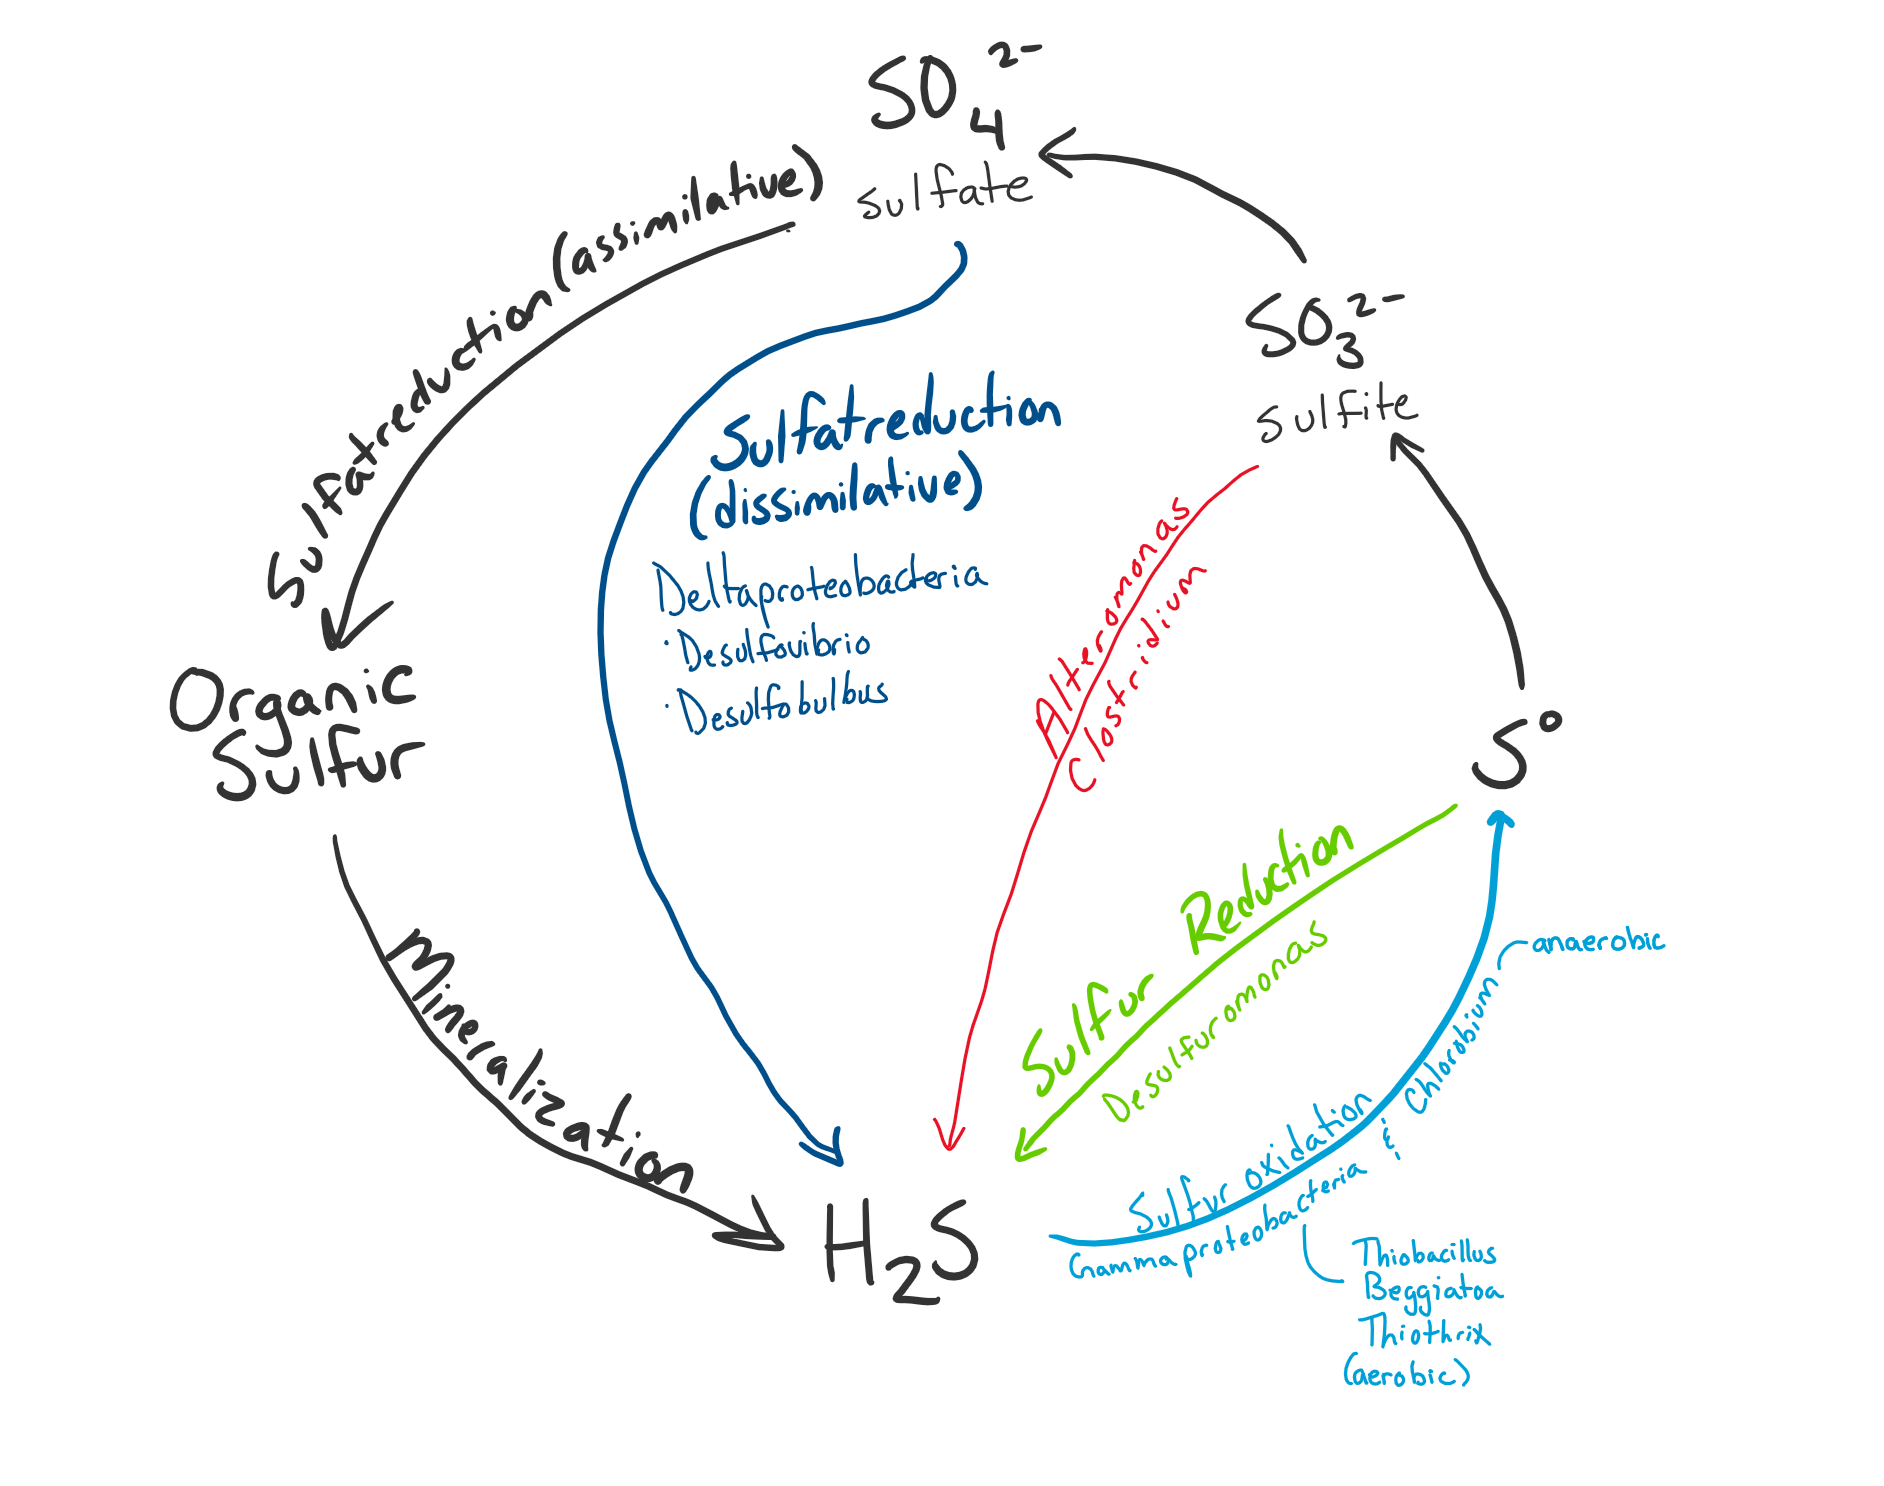
\includegraphics[width=0.85\textwidth]{figures/Sulfur_Cycle_for_Hydrothermal_Vents.png}
            \caption{Basic reactions in sulfur cycle} 
            \label{fig:micr_ecol_a}
         \end{subfigure}%
         
         \hspace*{\fill}   % maximize separation between the subfigures

         \begin{subfigure}{0.85\textwidth}
            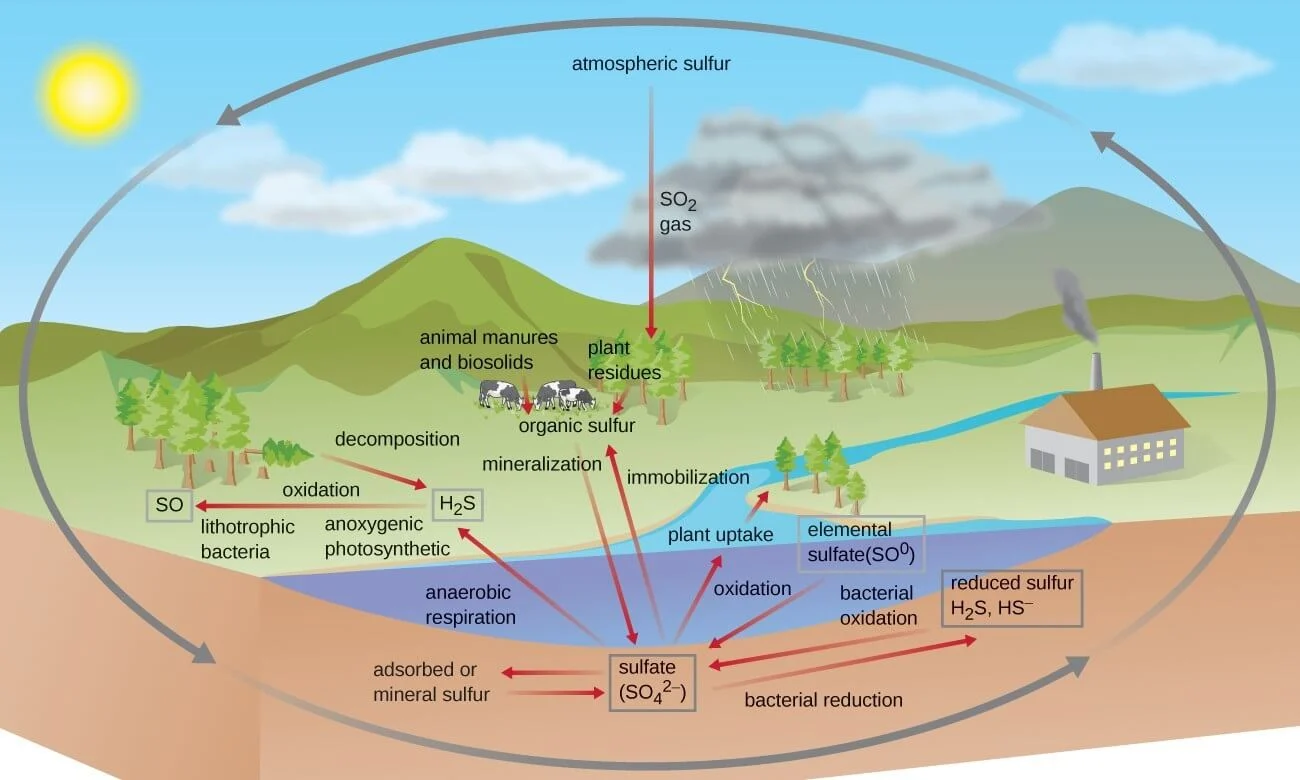
\includegraphics[width=0.85\textwidth]{figures/sulfur_village.png}
            \caption{Sulfur cycle reactions per environmnetal type} 
            \label{fig:micr_ecol_b}
         \end{subfigure}%
         
         \hspace*{\fill}
         
         \caption[The cycle of S and the role of microbial communities]{
            The cycle of sulfur (S) (up) and the contribution of microbial communities on it (down, image source: \href{https://openstax.org/resources/3002d0fba25221d24455917117482a079a11f321}{OpenStax}).
            % Marine microbial communities contribute to CO$_2$ sequestration, nutrients recycle and thus to the release of CO$_2$ to the atmosphere. 
            % Soil microbial communities decomposers organic matter and release nutrients in the soil 
            % from \citep{cavicchioli2019scientists} doi: \href{https://doi.org/10.1038/s41579-019-0222-5}{10.1038/s41579-019-0222-5}, under \href{http://creativecommons.org/licenses/by/4.0 license}{Creative Commons Attribution 4.0 International License}
         }
         \label{fig:co2}
      \end{figure}

      The biological fluxes of most of the major elements (i.e., carbon, hydrogen, oxygen, nitrogen and sulfur) required
      for any biological macro-molecule,
      are driven largely
      by microbially catalyzed, thermodynamically constrained redox reactions~\citep{falkowski2008microbial}. 
      Phosphorus the last of the 6 fundamental elements for life, is also included in the metabolic pathways catalyzed by microbes. 
      Thus, microbial communities consist of hundreds or even thousands of metabolically diverse strains and species~\citep{leventhal2018strain},
      and their functions
      and determine the fitness of most organisms on Earth. 
      In case of human health, specific microbial enzymatic pathways and molecules necessary for health promotion have been well known.
      Some of these "beneficial factors" are already known for probiotics and species in the human microbiome~\citep{marco2021defining}.

      The relationship between the taxonomic and the functional profile of a microbial community
      has been an open question for scientists; is the \textit{who} or the \textit{what} more important
      to distinguish communities~\citep{xu2014more}?
      And how does each of these profiles respond to the various perturbations of an environment; 
      Do they tend to converge~\citep{estrela2022functional}?
      Do perturbations of the taxonomic composition of a community influence the robustness of the community’s functional profile~\citep{eng2018taxa}?
      divergence of each under  
      and from an evolutionary point-of-view. 
      Does it matter \textit{who} is doing \textit{what} and how does this affect 
      the niche of a species~\citep{louca2018function}?  
      And what about the rare taxa and their corresponding functions in an assemblage~\citep{chen2020rare, jousset2017less}?

      % MICROBIAL ECOLOGY and OPEN QUESTIONS 
      % \if 0
      % \myparagraph{Microbial Ecology}
      % \fi
      \paragraph{Microbial Ecology} focuses on the study of the following interactions: 
      \begin{itemize}
         \setlength\itemsep{0.05em}
         \item those between microbial taxa and their environment
         \item those among the various microbial taxa present in a community, and
         \item those between microbial taxa and their host~\citep{isme}
      \end{itemize}

      Microbial ecologists also investigate the role of microbial taxa in 
      biogeochemical cycles~\citep{falkowski2008microbial} and their interaction 
      with anthropogenic effects e.g. pollution and climate change~\citep{cavicchioli2019scientists}.

      Even though HTS has allowed a massive extension of our knowledge in  
      specific enzymatic reactions that regulate these pathways the rules that determine 
      the assembly, function, and evolution of these microbial communities remain unclear. 
      Thus, both in case of environmental and human
      the underlying mechanisms for how microbial assemblages work and affect their environment, remain to be discovered.
      Understanding the underlying governing principles is central to microbial ecology~\citep{giri2021metabolic} and crucial for designing microbial consortia for biotechnological~\citep{giri2020harnessing} or medical applications~\citep{kong2018designing}.

      Studies such as the one of~\citeauthor{louca2016decoupling}
      have opened new frontiers in our understanding on microbial assemblages. 
      After building metabolic functional groups and assigning more than 30,000 marine 
      species to these groups,~\citeauthor{louca2016decoupling} showed 
      that the distribution of these functional groups were influenced by environmental 
      conditions to a great extent, shaping \textit{metabolic niches}.
      At the same time though, the taxonomic composition within individual functional groups
      were not affected by such environmental conditions~\citep{louca2016decoupling}.

   % MICROBIAL INTERACTIONS INTRO
   % \if 0fector models describe how species abundance (x) variation depends on metabolite conce
   \subsection{Ecological interactions in microbial communities}
   \label{subsec:ecol_interactions}
   
      Moreover, to elucidate how these assemblages work the biotic interactions have to be 
      considered too. 
      Microbial interactions play a fundamental role in deciphering the underlying mechanisms that govern ecosystem functioning \citep{braga2016microbial, faust2012microbial}. 
      Microbes secrete costly metabolites (called \textbf{byproducts}) to their environment, 
      which other microbes can absorb and exploit~\citep{pacheco2019costless}.
      By exchanging metabolic products, mostly as there are also other ways of interactions 
      e.g. quorum sensing, microbial taxa establish various interactions. 
      
      The interaction between two taxa can either be neutral or 
      positive / negative (Figure~\ref{fig:micro-inter-types}).
      In case of a positive interaction, 
      there is a case where both taxa benefit one from another.
      This \textit{win-win} relationship is called \textbf{mutualism} (or "cooperation")
      and it can be a result of
      \textit{cross-feeding}, in which two species exchange metabolic products~\citep{faust2012microbial}.
      Such is the case in biofilms where multiple bacterial taxa are working together  
      building a structure that provides them antibiotic resistance~\citep{santos2019evolutionary}.
      There is also the case where only one of the two taxa
      benefits without helping or harming the other; 
      this interaction is called \textbf{commensalism}~\citep{faust2012microbial}. 
      For example, \textit{Nitrosomonas} oxidize ammonia (NH$_3$) into nitrite (NO${_2}^{-}$), so  
      \textit{Nitrobacter} can use it to obtain energy and oxidize it into nitrate (NO${_3}^{-}$)~\citep{laanbroek2002nitrite}.
      Such interactions are quite common in microbial communities.

      \begin{figure}[!h]
         \centering
         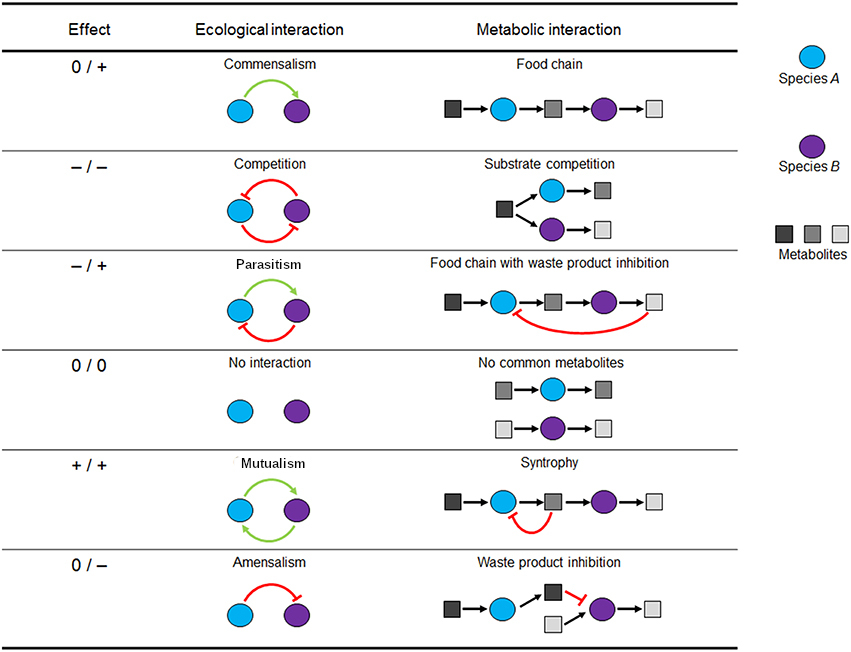
\includegraphics[width=.9\textwidth]{figures/interaction_types.jpg}
         \caption[Microbial interactions types]{Microbial interaction types along 
         with their corresponding metabolic ones.
         Due to certain metabolic interactions, two taxa may have a positive, a negative
         or a neutral effect one another. 
         Figure based on \citep{perez2016metabolic}}
         \label{fig:micro-inter-types}
      \end{figure}

      In case of a negative interaction, can harm each other either way (\textbf{compe-tition}). 
      That is the case between 
      \textit{Listeria monocytogenes} and \textit{Lactococcus lactis} in the study of~\citeauthor{freilich2010large} where their resource competition is high enough
      contributing to their non-overlapping existence~\citep{freilich2010large}.
      Moreover, similarly to commensalism, 
      there is also the case when a taxon has a negative affect on the other
      without getting any harm (\textbf{amensalism}). 
      Such is the case for \textit{Acidithiobacillus thiooxidant} that produces
      sulfuric acid (H$_2$SO$_4$) by oxidation of sulfur~\citep{bobadilla2013stoichiometric} which is responsible for lowering of pH in the culture media which inhibits the growth of most other bacteria~\citep{jin2018ph}.
      Finally, one of the taxa may have a positive affect (host) on the other, but the 
      latter (parasite) can be harmful to its benefactor (\textbf{parasitism})~\citep{faust2012microbial}. 
      There are multiple cases of parasitism in real-world communities; 
      species of the genus \textit{Bdellovibrio} for example, are parasites of other (gram-negative) bacteria~\citep{stolp1979interactions}.

      However, we have a very limited understanding
      of such interactions and the ways that are combined to
      rule community-level behaviors. 
      Thus, we cannot predict community responses to
      perturbations (community stability)~\citep{venturelli2018deciphering}.
      Over the years, various methods have been used to infer such interactions. 
      co-occurrence modells~\citep{faust2012microbial},
      time series data and causal models~\citep{mainali2019detecting},
      through metabolic interactions as proxy~\citep{levy2012reverse}.
      Dynamic models, such Ordinary Differential Equations (ODEs)
      and the Generalized Lotka–Volterra (gLV) model~\citep{gonze2018microbial}
      have been also widely used. 
      Finally, in recent years, 
      metabolic networks and constraint-based models have been also used
      to predict microbial interactions~\citep{heinken2021advances, dukovski2021metabolic}.
      This last approach allows predictions for the metabolic dynamics of the community 
      as well as of the exact set of compounds the taxa of the community exchange~\citep{levy2012reverse}.
      Still though, microbial interactions inference is a challenging task 
      and several questions are still open. 
      
      Apparently, the environmental conditions affect the ecological interactions to a
      great extent. 
      A pair of taxa may be competitors in one case but have a neutral interaction in another one. 
      In addition, evolutionary processes may change certain interactions; 
      for example moving from commensalism to parasitism~\citep{parmentier2016commensalism}.
      Both ecological and environmental interactions 
      play a part in the composition and the functional potential of 
      microbial assemblages. 
      On top of that, pairwise microbial interactions can be modified by a third organism, 
      leading to higher-order effects that influence community behaviors~\citep{bairey2016high}. 
      % Ecological driver species, which exhibit a large impact on community structure and function, represent key nodes in the network that could be manipulated 
      % to control community states~\citep{gibson2016origins}.
   \subsection{Reverse ecology: transforming ecology into a high-throughput field}
   \label{subsec:revec}

      For decades, \textit{reductionism} has been the main conceptual approach 
      in biological research~\citep{noble2008music}.
      Traditionally, for studies relating genetics and ecology
      scientists first identify an ecological adaptive phenotype 
      and then they try to detect causal genetic variation~\citep{noble2008music}.
      However, as described in the previous sections, HTS data have turned the page in 
      Biology research in numerous ways. 
      Therefore, it is nowdays possible to \textit{reverse} this framework and by 
      using the genomic information retrieved, to study 
      the ecology of a species.
      The \textbf{Reverse Ecology} framework uses advances 
      in both systems biology and genomic metabolic modeling to implement  
      community ecology studies 
      with no a priori assumptions about the organisms under consideration~\citep{cao2016revecor}.
      Therefore, Reverse Ecology 
      attempts to interpret HTS (genomic) data as large-scale ecological data~\citep{levy2012reverse}.

      \begin{figure}[!h]
         \centering
         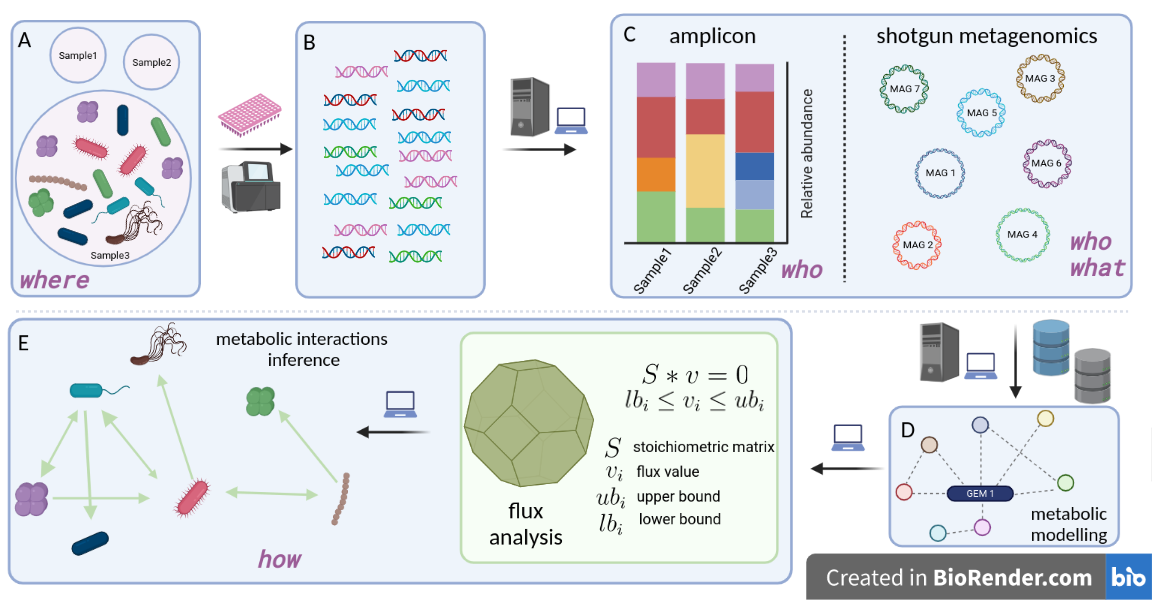
\includegraphics[width=135mm]{figures/reverse_ecology.png}
         \caption[The \textit{Reverse Ecology} framework.]{Without any previous knowledge of the species present in a community (A) and using HTS data (B) one can have an overview of the species present 
         as well as in the functional profile of the community (C).
         Especially when the complete genome of a species has been retained (either using 
         metagenomics (MAG) or using targeted approaches to get this (SAG))
         researchers can build its corresponding GEM (D) and then 
         infer the ecology of a taxon predicting 
         the exogenously acquired compounds as well as ecological interactions between the taxon under study and other species present in a community (E). 
         Both network topology - and constraint - based methods can be used to this end.
         Created with \href{BioRender.com}{BioRender.com}.
         }
         \label{fig:revecol}
      \end{figure}

      As shown in Figure~\ref{fig:revecol}, the Reverse Ecology framework 
      has multiple alternatives and various methods can exploit this concept.
      The analysis of metabolic networks (see Section~\ref{chap:dingo}) 
      plays a great part in several Reverse Ecology approaches.
      Most parts of this dissertation have been influenced by this, especially 
      chapters~\ref{cha:prego},~\ref{chap:dingo} and~\ref{cha:swamp}.
      


% SECTION 2

\section{High Throughput Sequencing in Microbial Ecology}

      % SUBSECTION 1.1.2 
   \subsection{'Omics methods to access the \textit{who} and the \textit{what}}
   \label{subsec:omics}
      To discover the microbial taxa present in a sample, scientists have 
      explored multiple ways through the years. 
      Only a particularly limited proportion of the microbial species 
      can be cultured~\citep{steen2019high}.
      Therefore, mono-cultures and enrichment cultures allow us to observe 
      only a small fraction of the actual diversity. 
      As a consequence, other methods for the taxonomic identification of theses
      species are required.
      Based on molecular characteristics of the microbial taxa, 
      over the last decades, a series of methods have been developed. 
 
      Moving from single species to assemblages, molecular-based identification and functional 
      profiling of communities has become available through marker (metabarcoding), 
      genome (metagenomics), or transcriptome (metatranscriptomics) sequencing from environmental 
      samples \citep{goldford2018emergent}. 
      To a great extent, these methods address the problem of how to produce and get access 
      to the information on different biological systems and molecules.

      In case that the taxonomic assessment of a sample is the aim of a study, 
      \textit{metabarcoding} (amplicon-targeted metagenomics) and \textit{shotgun metagenomics} can be used as alternative options. 
      Metabarcoding studies are common, well-established, cheaper and less computationally demanding than shotgun metagenomics~\citep{bell2021comparing}. 
      Its primary drawbacks are the limited information present in the short barcoding sequence and the possible taxonomic bias arising from differential efficiency of PCR primer pairing in different species~\citep{blazewicz2013evaluating}. 
      On the other hand, shotgun metagenomics offers a better taxonomic resolution at the species level by obtaining information from random sampling of virtually all genomic regions, and can address microbiome metabolic functions and entire biochemical pathways~\citep{sharpton_introduction_2014}. 
      Unfortunately, it requires higher sequencing coverage and, consequently, more complex and demanding downstream bioinformatics analysis~\citep{laudadio2018quantitative}. 
      Nevertheless, it has recently been suggested that shotgun metagenomics provides a deeper characterisation of microbiome complexity that metabarcoding recently enabling to profile up to the level of strains, whose non-core genome is responsible for crucial functional differences within the same species, 
      as the fundamental units of the community~\citep{davila2019review, clooney_comparing_2016, segata_road_2018}.       
      
      Targeting community composition and functional profiles in several ecological niches, 
      microbial ecologists produce vast 
      amount of sequencing data~\citep{harrison2021european}.
      These approaches enable the study of ecosystems with no prior knowledge of the resident species, 
      while at the same time a number of challenges for their management and bioinformatics analysis is rising. 
   \subsection{Bioinformatics challenges in the analysis \& management of HTS data}
   \label{subsec:hts_chal}

      Moving from raw data to taxonomic and functional profiles of a microbial community comes with high computational costs, especially in the case of metagenome studies~\citep{yang2021review}.
      Sequence pre-processing, assembly, classification, and functional annotation consist of several steps the most of which a significant number of algorithms or/and software tools are available~\citep{breitwieser2019review, roumpeka2017review}. 
      Tailoring each tool's execution parameters to reflect each experiment's idiosyncrasy is vital for legitimate findings, yet it makes analyses of metagenomics data even more complex. 

      In addition, there are several challenges on the bioinformatics analysis \textit{per se}.
      \textit{Taxonomy assignment} in both amplicon- and shotgun metagenomics studies 
      has several issues to meet~\citep{simon2019benchmarking};
      the taxonomy of microbes is a challenge per on its own~\citep{parks2020complete}.

      In amplicon studies, among the most major issues is the one of the abundances of the
      taxa found~\citep{fonseca2018pitfalls, balint2016millions} as well as the presence of pseudo-genes~\citep{song2008many}.
      In the first case, 
      % a number of 
      issues such as  
      % \begin{itemize}
      %    \setlength\itemsep{0.05em}
         % \item 
      the usually unknown number of marker gene copies per cell in the various taxa,
         % \item 
      PCR - related biases such as primer-template mismatches, length difference of amplicon, artificial base changes, chimeric molecules 
         % \item 
      and library preparation - related issues such as chimera formation by the mix of amplicons from different samples
      % \end{itemize}
      makes hard for the method to have robust quantitative results~\citep{balint2016millions}. 
      Reads on the other hand resulting from pseudo-genes or/and highly divergent nuclear mitochondrial pseudo-genes (NUMTS), nonfunctional copies of mtDNA in the nucleus that have been found in major clades of eukaryotic organisms~\citep{bensasson2001mitochondrial}, 
      can lead either to false positive taxonomic hits or to non-hits at all,
      adding extra noise to the amplicon results returned.

      In shotgun metagenomics studies there are also several challenges. 
      Meta-genome \textit{assembly} comes with a great number of challenges. 
      Due to the uneven (and unknown) representation of the different organisms within a metagenomic mixture, simple coverage statistics can no longer be used to detect the repeats, while unrelated genomes may contain
      nearly-identical DNA (inter-genomic repeats) representing, for example, mobile genetic elements~\citep{ghurye2016focus}.
      At the same time, \textit{binning} is a rather tricky step too; 
      several algorithms have been developed to address it~\citep{yue2020evaluating}
      while approaches combining the output of individual algorithms have been introduced too~\citep{song2017binning_refiner}.


      The vast amounts of data that come with metagenomic studies and the computational complexity for implementing multiple steps mentioned earlier imply immense computational requirements for their analysis that usually exceed the capacity of a standard personal computer~\citep{merelli2014managing}. 
      % 
      % Therefore, several pipelines were established to address the challenges of the bioinformatics analysis of metagenomes. 
      % In addition, as such analyses exceed the capacity of a standard personal computer, it is essential for the researchers to ensure access to  
      % computing infrastructures that will support their needs.
      % Computing infrastructures may range from a local server of an individual lab to High-Performance Computing (HPC) or/and cloud solutions adopted at the (inter)national level, such as the \href{https://eosc-portal.eu}{EOSC} and 
      % \href{https://www.embassycloud.org}{EMBL-EBI Embassy Cloud}. 
      % 
      % The swift pace of establishing new algorithms and software as well as new versions of already published ones makes software versioning an essential issue for FAIR microbiome bioinformatics analyses. 

      \paragraph{For HTS data to be available }
      to the scientific community for further exploitation,
      it is required to be accompanied by
      comprehensive metadata~\citep{vangay2021microbiome}. 
      The potential of HTS data is revealed when they are available to the community; 
      this way studies that could never been performed
      by individual researchers, labs or institutes are now possible. 
      This way, 
      a single researcher can now investigate
      how a certain environmental type reacts in response to an environmental 
      variable by making use of hundreds of metagenomic samples 
      that fulfill the criteria of his/her study.
      Finding data of interest however, can be particularly difficult.
      This is so because of a combination of reasons.
      HTS data can be particularly heterogeneous based on both the data generation and the data processing methods used. 
      However, it is mostly the vague or even absent metadata accompanying the HTS data set several limitations in their re-usage~\citep{hu2022challenges}. 

      The concept of FAIR data (Findability, Accessibility, Interoperability \& Reuse)
      and the \href{https://www.go-fair.org/fair-principles/}{FAIR principles}\footnote{\href{https://www.go-fair.org/fair-principles/}{https://www.go-fair.org/fair-principles/}}
      along with community - driven standards and resources such as 
      the \href{https://gensc.org/}{Genomic Standards Consortium (GSC)}\footnote{\href{https://gensc.org/}{https://gensc.org/}},
      the Minimal Information about any Sequence (MIxS)~\citep{yilmaz2011minimum, yilmaz2011genomic}
      and the \href{https://microbiomedata.org/metadata/}{National Microbiome Data Collaborative (NMDC)}\footnote{\href{https://microbiomedata.org/metadata/}{https://microbiomedata.org/metadata/}}~\citep{wood2020national}
      aim to address these challenges~\citep{wilkinson2016fair}.
\section{Data integration in the service of microbial ecology}

   \subsection{Moving from \textit{partial} to more \textit{comprehensive} data interpretation}
   \label{subsec:integration_intro}
      Over the last decades, based on
      computational and mathematical analysis and modeling,
      and by exploiting interdisciplinary data and knowledge, 
      Systems Biology focuses on complex interactions within biological systems~\citep{tavassoly2018systems}.
      The more data becoming available from all the different levels
      of hierarchy of life, the more feasible for scientists to 
      move from reductionism to more holistic approaches 
      for interpreting how the properties of a system emerge~\citep{noble2008music}.

      Microbial ecology as a field would have not been the same if it was not 
      for resources such as 
      Integrated Microbial Genomes (IMG) and GOLD~\citep{chen2021img}, 
      SEED and the Rapid Annotation of microbial genomes using Subsystems Technology (RAST)~\citep{overbeek2014seed}, 
      Pathosystems Resource Integration Center (PATRIC),
      ~\citep{zhulin2015databases}
      and many more that thousands of researches use in their every day work. 
      All these approaches, regardless on what they focus, they are all based on data aggregation and data integration approaches. 
      \textit{Data aggregation} denotes the gathering of data from diverse sources
      in a certain scheme that will allow them to be used as a combined data-set for 
      further analysis~\citep{simpson2010secure}. 
      In case of microbial ecology, that means that data focusing on the genetic 
      information can be combined with phenotypical data or even with environmental and 
      ecological data.
      \textit{Data integration} on the other hand, is the process of combining everything
      retrieved on the data aggregation step, 
      to get a summarization and unified view of all the accumulated data~\citep{schneider2012teaching}.
      Such summarizations may lead researchers to new hypotheses that 
      in turn, will be tested through new experiments (Figure~\ref{fig:data_int}).


      \paragraph{Data integration comes with great challenges.}

      Apparently, data integration methods are based on the existence of primary databases. 
      Each of these database resources come with its own assumptions and schemas. 
      Therefore, it is not a straight-forward task to recognize or assign and maintain 
      the correct names of biological entities across the various databases~\citep{stein2003integrating}.
      Taxonomy is quite an indicative example. 
      As there is no a global taxonomy system, even the species name can be a 
      great challenge in such approaches; how to retrieve information about a species
      that does not have the same name on the various databases to integrate? 
      Therefore, retrieving and mapping entities can be rather complex.  
      Similarly to taxonomy, most biological databases are constantly changing. 
      Thus, integration approaches need to be periodically so the always keep updated~\citep{stein2003integrating}.
      In addition to the heterogeneity of the data \textit{per se},
      further challenges that make data integration even harder in case of biological data,
      is the lack of unique standards~\citep{triplet2011systems}.
      In the case of HTS data, great efforts to address this challenge have been 
      made (see Section~\ref{subsec:hts_chal}).

      \begin{figure}[!h]
         \centering
         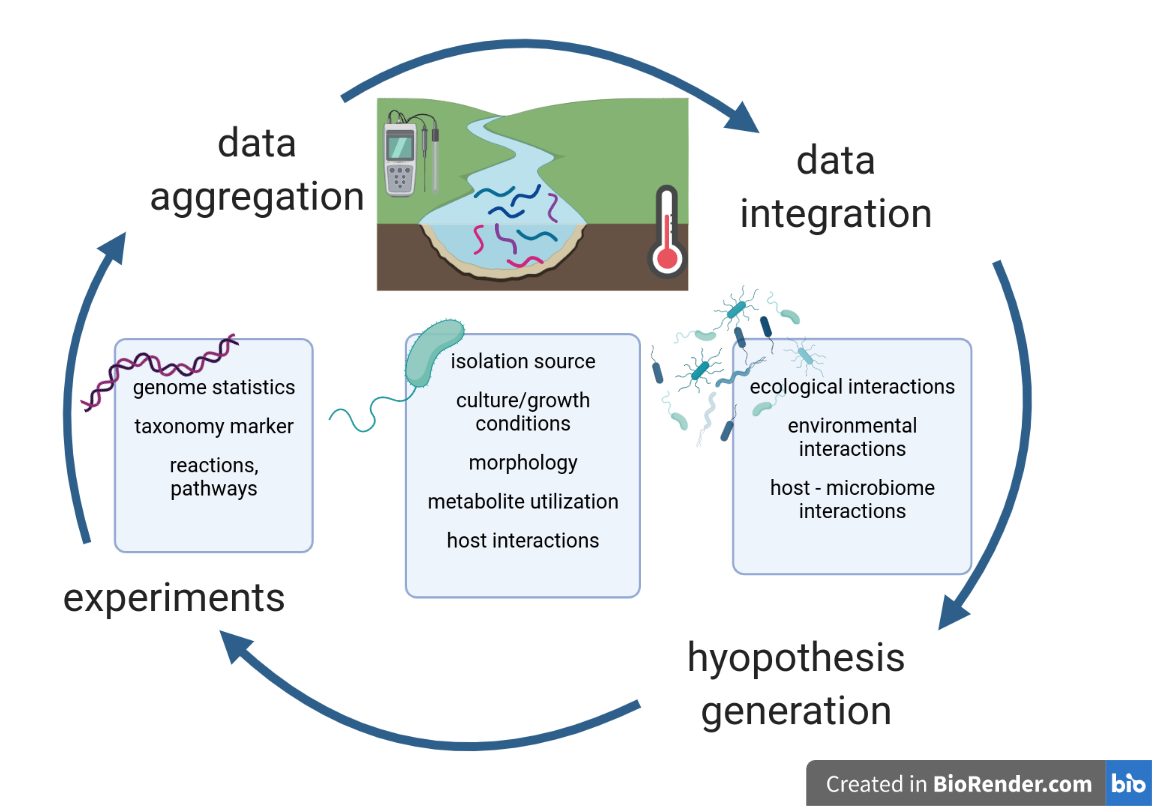
\includegraphics[width=0.95\textwidth]{figures/data_integration_scheme.png}
         \caption[Data integration in Microbial Ecology]{A data integration scheme for microbial ecology oriented data. 
         Measurements from experiments at every level of organization of life are gathered and their summary provides researchers with new insight. Created with \href{BioRender.com}{BioRender.com}.
         }
         \label{fig:data_int}
      \end{figure}


      One of the most typical examples of data integration and its potential
      is the \href{https://www.string-db.org/}{STRING database}\footnote{\href{https://www.string-db.org/}{https://www.string-db.org/}}, where multiple channels of information are combined 
      to retrieve protein - protein interactions~\citep{mering2003string, szklarczyk2021string}. 
      In addition to databases of interaction experiments and others of interaction predictions, text-mining methods of the scientific literature enhance further the 
      PPI predictions~\citep{szklarczyk2021string}.
      Focusing on bacterial information, \href{https://bacdive.dsmz.de/}{BacDive}\footnote{\href{https://bacdive.dsmz.de/}{https://bacdive.dsmz.de/}}~\citep{reimer2019bac}
      is a great example - resource of the added value that data integration methods can provide. 

      \paragraph{Multiple integration approaches} attempt to address the challenges described. 
      The \textit{data warehousing} approach is a widely used data integration approach and has two mains steps; 
      first, a unified data model that can accommodate all types of  
      information from the various source databases is schemed.
      Then, software is developed aiming at  
      gathering the data from the source databases, 
      convert them to match the unified data model and 
      then load them into the warehouse~\citep{stein2003integrating}.
      Once these steps have been completed, further analysis of the once
      several bits of information - now a single data-set, can be performed.
      New insight may come up either from statistical analyses on the unified
      data-set or from their visualization~\citep{leonelli2013integrating}.  

   \subsection{Ontologies \& metadata standards: cornerstones for efficient data integration}
   \label{subsec:metadata_intro}
      Data integration in general, 
      is strongly dependent by the extent that standards are used. 
      Especially in case of vast and heterogeneous data, 
      data integration cannot return valid results 
      when there is not a certain way
      of denoting the entities included.
      Thus, it is dependent on the way data are distributed in the fist place 
      as well as on whether their content follow certain principles or not. 
      To address these challenges, several ontologies and standards have 
      been established through the years, trying to cover all the different 
      types of needs of the microbial ecology community. 

      According to~\citeauthor{stevens2000ontology} an \textit{ontology} is the \textit{"concrete form of a concepcualisation
      of a community's knowledge of a domain"}~\citep{stevens2000ontology}.
      Ontologies attempt to capture the main concepts in a \textit{knowledge domain}, 
      i.e. a body of knowledge that is often associated with a
      specialized scientific discipline. 
      For example, considering \textit{where} a species live or \textit{where} a process occurs, one need to describe the environment where the phenomenon under study 
      takes place. 
      Thus, the \href{https://sites.google.com/site/environmentontology}{Environment Ontology (ENVO)}\footnote{\href{https://sites.google.com/site/environmentontology}{https://sites.google.com/site/environmentontology}} aims to provide descriptions of environments~\citep{buttigieg2016environment}.
      Using sets of entities, meaning entities sharing several attributes (\textit{concepts}), 
      descriptions of the interactions between concepts (\textit{relations}), 
      entities - members of a concept (\textit{instances}) and 
      properties of relations that aim to constrain the value a class or an instance may get (\textit{axioms}) aim to create an agreed vocabulary and
      semantic structure for exchanging
      information about that domain~\citep{stevens2000ontology}. 
      A \textit{vocabulary} includes definitions and an indication of how concepts are inter-related which collectively impose a structure on the domain and constrain the
      \citep{uschold1998enterprise}.
      Ontologies are fundamental for data integration as they ensure that the knowledge
      included in a text or in a data set, can be captured by both humans and computers. 


      \paragraph{Metadata are essential for most if not all types of data.} 
      Consider sampling from a set of healthy and patients. 
      Then what if you do not know what samples are coming from each group? 
      You data have been already degraded. 

      In a recent study~\citeauthor{furner2020definitions} gave a list of several definitions of metadata.
      The one of~\citeauthor{zeng_qin_2016} is probably the more inclusive one:
      \textit{"
      Structured, encoded data that describes characteristics of information-bearing entities
      (including individual objects, collections, or systems) to aid in the identification,
      discovery, assessment, management, and preservation of the described entities."
      }
      \textit{Structured} are data that are highly organized and easily decipherable by machine learning algorithms while
      \textit{encoded} are those that have been converted into digital signals.

      Moreover, for the most efficient design and implementation 
      but also to ensure the Interoperability of structured metadata 
      across various computing systems and environments, 
      a range of \textit{standards} have been developed.  
      % \textit{Metadata standards} focus on 
      % data structure (\textit{schemas}), content, value, data format.
      \textit{Data structure (schemas) standards} and
      rules for formatting the contents of metadata records 
      along with
      \textit{encoding} and \textit{exchange} standards 
      are combined to build up metadata.

      As mentioned in Section~\ref{subsec:hts_chal}, great efforts have been 
      made on setting 
      HTS - related metadata standards~\citep{yilmaz2011minimum, yilmaz2011genomic, wood2020national}.
      That is so because comprehensive metadata is the only 
      way to ensure:
      \begin{itemize}
         \setlength\itemsep{0.05em}
         \item humans will be able to contextualise where and how the data originated as well as how they were analysed
         \item computing systems will be able to exploit this metadata provenance further
      \end{itemize} 
      Thus, 
      details regarding \textit{when}, \textit{where} and \textit{how} samples were collected 
      can be provided. 
      Moreover, these metadata may align against community developed standards where possible. 
      For example, addressing the question of \textit{where} a sample was collected, 
      the answer could be \textit{"lake"} or \textit{ENVO:00000020}.
      The difference in terms of computer science is huge; 
      it is probably trivial for a human to think that a \textit{lake} is an aquatic
      environment and in fact a freshwater one. 
      However, it is only the \textit{relations} of an ontology that would allow 
      a computer to come up with the same "conclusions". 



      Regarding the environmental metadata of a sample, 
      ENVO~\citep{buttigieg2016environment} and MIxS~\citep{yilmaz2011minimum}
      are working together to build a solid framework~\citep{environmentontology_2021}. 
      The \textit{broad-scale environmental context} value is representing the 
      major environmental system a sample came from;
      thus, \textit{\href{http://purl.obolibrary.org/obo/ENVO_00000428}{biome}}~\footnote{\href{http://purl.obolibrary.org/obo/ENVO_00000428}{http://purl.obolibrary.org/obo/ENVO\_00000428}} 
      ENVO terms should be used as values. 
      An ENVO \textit{biome} term represents an ecosystem to which resident ecological communities have evolved adaptations.
      The \textit{local environmental context} value, stands for 
      entities which are in a sample's local vicinity and may have significant causal influences on the sample; 
      ENVO \textit{feature} terms may be used for that.
      Finally, 
      as values of the \textit{environmental medium} 
      category, 
      environmental \textit{\href{http://purl.obolibrary.org/obo/ENVO_00010483}{material}}~\footnote{\href{http://purl.obolibrary.org/obo/ENVO_00010483}{http://purl.obolibrary.org/obo/ENVO\_00010483}} (one or more) 
      immediately surrounded 
      the sample prior to sampling.
      However, other resources 
      use different schemes for describing the environment of a sample.
      For example in the GOLD database~\citep{mukherjee2021genomes},
      a five-level ecosystem classification path that includes 
      Ecosystem, Ecosystem Category, Ecosystem Type, Ecosystem Subtype and
      Specific Ecosystem
      has been adopted. 

      Besides the environmental metadata that describe the origin of the sample,
      the sequencing technology used (in case of raw data)
      along with metadata about the
      the computational steps implemented 
      and a thorough description of the results retrieved, for example  
      taxa found to be linked to a taxonomy scheme (in case of processed data)
      are required. 
      
      Figure~\ref{fig:metadata_examples} highlights both the potential and the 
      challenges related to HTS - oriented metadata. 
      Metadata describing the sample in case~\ref{fig:metadata_examples_a}
      are limited and neither a human nor a computer is able to 
      capture the actual environment from where the sample was collected. 
      In the~\ref{fig:metadata_examples_b} case, accompanying metadata are clearly
      more informative.
      Both a human and computing systems, can capture that the sample comes from 
      an \textit{oceanic epipelagic zone biome} (\href{http://purl.obolibrary.org/obo/ENVO_01000035}{ENVO\_01000035})
      and more specifically
      \textit{oligotrophic water} (\href{http://purl.obolibrary.org/obo/ENVO_00002223}{ENVO\_00002223}).
      However, two of the challenges for HTS metadata are demonstrated in this case;
      first, the use of \textit{Deep Chlorophyll Maximum} 
      denotes the need for extra terms to be added in ENVO.  
      On top of that, the need for extra training of the community in these methods
      is shown as the the ENVO term denoting \textit{oligotrophic water} 
      should be provided as the \textit{feature} 
      and \textit{Deep Chlorophyll Maximum} should be used to 
      describe the \textit{material}.


      \if 0 
      To define biome - feature - material, have a look a this
      https://www.ddbj.nig.ac.jp/faq/en/biome-feature-material-e.html
      \fi
      
      \begin{figure}[!h]

         % \hspace*{-1.2in}
         \centering

         \begin{subfigure}{0.72\textwidth}
           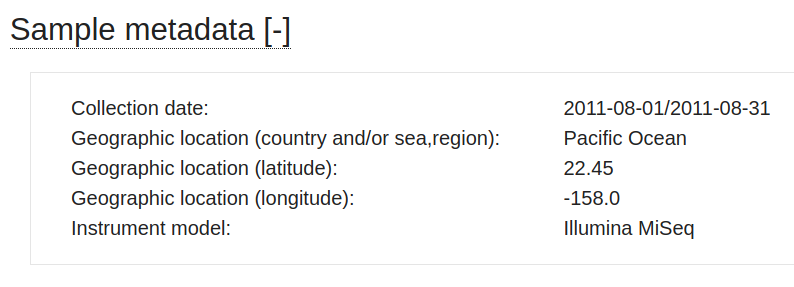
\includegraphics[width=\linewidth]{figures/SRS1753450_metadata.png}
           \caption{Poor, non machine readable metadata} \label{fig:metadata_examples_a}
         \end{subfigure}%
         
         \hspace*{\fill}   % maximize separation between the subfigures
         
         \begin{subfigure}{0.72\textwidth}
           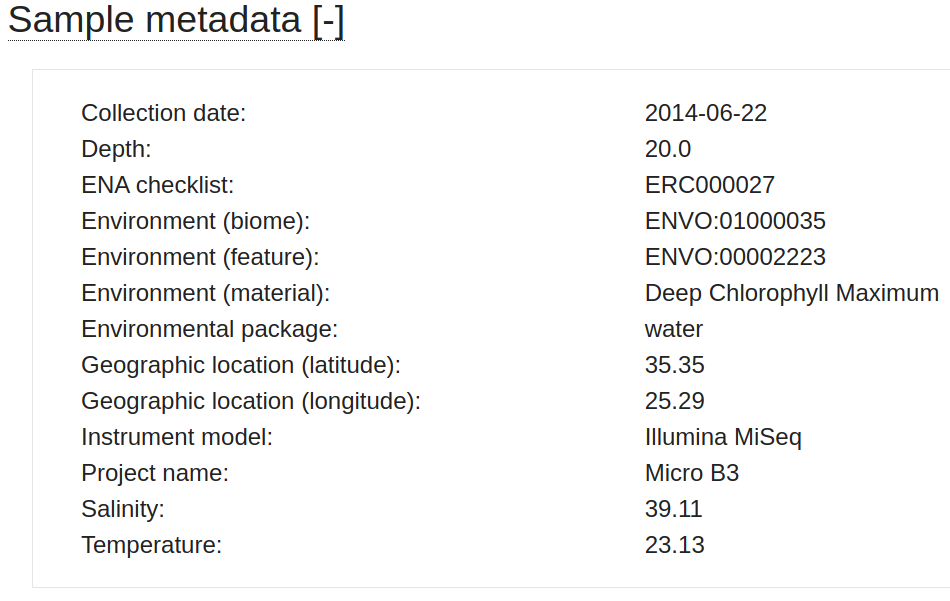
\includegraphics[width=\linewidth]{figures/ERS667566_metadata.png}
           \caption{Rich, partially machine readable metadata} \label{fig:metadata_examples_b}
         
         \end{subfigure}
       
       \caption[Samples metadata examples MGnify]{Example cases of HTS - sequencing metadata. Metadata in case~\ref{fig:metadata_examples_a} fail to describe 
       the origin of the sample both to a human and a computer. 
       In case~\ref{fig:metadata_examples_b} further metadata have been added 
       while most environmental metadata are provided as ENVO terms. 
       } 
       \label{fig:metadata_examples}
      \end{figure}


      Challenges associated with metadata deposition 
      as the one described above,
      mean submitters: 
      may lack of training and outreach resulting 
      or they do not fully realise the importance of metadata and 
      how to comply with standards.
      On top of that, the non-existence of standards in many cases 
      or the use of more than one standards lead to extra complexity.
      Only by a concerted effort on the part of the database providers, and with the encouragement and support of the research community, will we be able to tame the explosion of biological data~\citep{stein2003integrating}.
\section{Metabolic modeling: an interface for the genotype - phenotype relationship}


   \subsection{Constraint-based modeling for the analysis of metabolic networks}
   \label{subesec:modling}

      The relationship between genotype and phenotype is fundamental allowing to elucidate 
      mechanisms that govern the physiology of a species as well as those 
      ruling at the community level
      ~\citep{morris2020linking}.
      Meta-
      bolism penetrates most of the different levels of living entities horizontally~\citep{schramski2015metabolic} and 
      while it reflects the genomic information it indicates 
      what is actually going on on a cell at a certain time
      as a response to genetic or environmental changes~\citep{lima2021role}.
      One can use the \textit{Reverse Ecology} framework (Section~\ref{subsec:revec})
      to move all the way from genomic information to metabolism and the environment and back.
      To this end, \textit{metabolic networks} and their analysis are essential. 
      The vast number of reaction taking place in a cell are interlinked 
      (the product of the first acts as the substrate for the next) 
      building up metabolic pathways,
      while their stoichiometry allows their mathematical representation. 
      The rate of turnover of molecules through a metabolic reaction is called \textit{flux}.
      The metabolic network of a species consists of the sum of all the reactions that 
      take place in its cell,
      while \textit{metabolic model} is its representation in a mathematical format (Figure~\ref{fig:met_net})\footnote{               
         The \textit{Escherichia coli} model of Figure~\ref{fig:met_net} can be found at:\\
            \href{http://bigg.ucsd.edu/static/models/e_coli_core.xml}{http://bigg.ucsd.edu/static/models/e\_coli\_core.xml}
      }. 
      We call \textit{Genome-scale metabolic models (GEMs)} incorporate the vast majority of the 
      processes that occur in a cell or an organism in a mathematical format~\citep{feist2009reconstruction}.



      \begin{figure}
         \hspace*{-1.75in}
         \begin{tikzpicture}
            \node[anchor=west, yshift=150]       
            at (current page.west) {
               \includegraphics[width=140mm]{
                  figures/e\_coli\_map_crop\_Transp}
            };
            
            \node[anchor=east, xshift=10pt, yshift=-75pt]               
            at (current page.east) {
               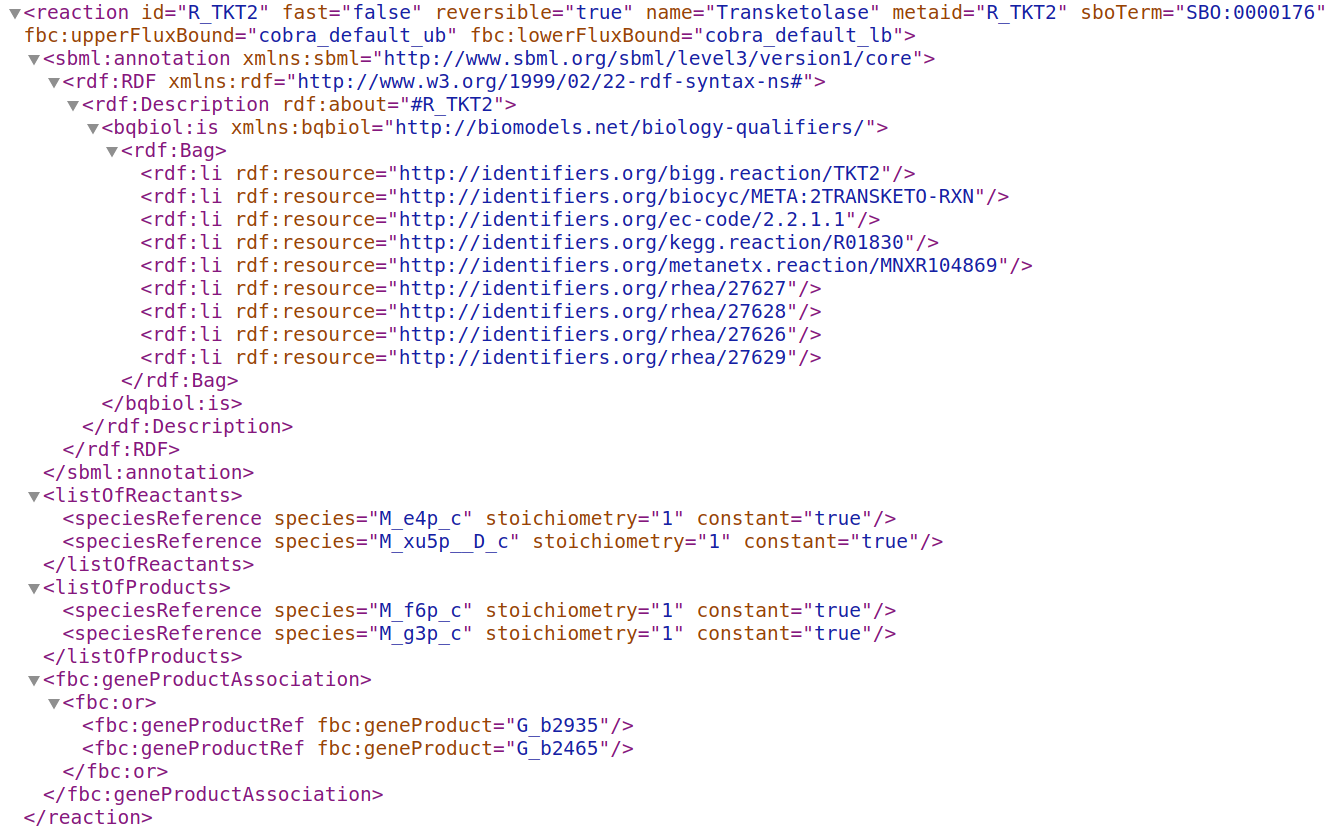
\includegraphics[width=148mm]{
                  figures/transketolase.png}
            };
 
         \end{tikzpicture}

         \caption[Part of the \textit{Escherichia coli} metaboic network and the Transketolase reaction]{
            Part of the \href{http://bigg.ucsd.edu/static/models/e_coli_core.xml}{\textit{Escherichia coli} BIGG metaboic network}  
            and the Transketolase reaction of it as integrated in the model}
         \label{fig:met_net}
      \end{figure}


      Once the complete genome is retrieved the enzymes and thus the potentially  
      catalyzed by the organism reactions can be listed. 
      However, the reconstruction of a GEM is not a straight forward task 
      and the more the complexity of the species increases, 
      the more effort is required for this task~\citep{thiele2010protocol}. 
      Thermodynamics, metabolome, physiological 
      and labelling data as well as literature can be also integrated in such models \citep{saldida2020unbiased}. 

      
      The analysis of GEMs has been interwoven with constraint-based modeling approachess~\citep{lewis2012constraining}.
      As all compounds are finite the concentration of each metabolite is bounded \citep{palsson2015systems}, meaning that the models derived from the
      metabolic networks have constraints.
      Likewise, as the laws of thermodynamics need to apply in such systems, 
      the flux of each reaction is also bounded.
      Therefore, the flux value of each reaction is constraint too.
      We call 
      \textit{steady state} the condition where the production rate of each metabolite equals its consumption rate~\citep{cakmak2012new}. 
      Equation~\ref{eq:intro} represents the main concept of constraint-based modeling at a steady state.
      \begin{equation}
      \label{eq:intro}
         \begin{split}
               S \cdot v = 0 , \\
               s.t.  v_{lb,i} \le v_i \le v_{ub, i}
         \end{split}
       \end{equation}
      where
      $S$ is a $m*n$ table ($m$ being the number of metabolites and $n$ the number of reactions of the model) 
      that stands for the \textit{stoichiometric matrix} of the model.
      The columns of $S$ consists of the  
      \textit{stoichiometric coefficients}, 
      i.e. the number of molecules a biochemical reaction consumes and produces,
      of the model's reactions.          
      $v \in \mathbb{R}^n $ is the \textit{flux vector} that contains the fluxes
      of each chemical reaction of the network. 
      As all the fluxes are bounded, for each coordinate $v_i$ of the vector $v$,
      there are constants $v_{ub, i}$ and  $v_{lb, i}$
      such that $v_{lb,i} \le v_i \le v_{ub, i}$, for $i \in [n]$, 
      where $n$ is the number of reactions of the model.
      The \textit{solution space} of systems such as the one of equation~\ref{eq:intro} 
      "live" in a \textit{\textbf{polytope}}.
      Further introductory material on computational 
      geometry can be found at Appendix~\ref{app:comp_geom_intro}.

      As discussed in~\citep{reed2012shrinking} a great range of constraints 
      govern the cells' operations; for a thorough overview on the constraints cells operate under, you may see~\citep{palsson2015systems}, Chapter $16.5$. 
      (Bio)physico-chemical- (e.g., thermodynamics, nutrient uptake, oxygen availability etc.) as well as connectivity-, capacity- and rates-related constraints 
      are applied on the functions of such a network.metabolic 
      Each of the aforementioned constraint categories include multiple constraints, such as 
      thermodynamics- and gene-expression-oriented constraints that add extra complexity 
      in the model. 
      The more constraints a model incoroporates, the more accurate the flux distributions it returns.

      Using constraint-based modeling scientists can 
      predict not only potential interactions,
      topology-based metabolic models are adequate for this task, 
      but also specific metabolic dynamics in a community~\citep{levy2012reverse}. 
      The most commonly used constraint-based methods for the analysis of metabolic networks
      are \textit{\textbf{Flux Balance Analysis (FBA)}}~\citep{orth2010flux} and 
      \textit{Flux Variability Analysis (FVA)}~\citep{gudmundsson2010computationally}.
      Both have been used to a great number of studies, providing fundamental isngight~\citep{ shastri2005flux,chapman2015flux}.
      Models estimate the minimum or the maximum of a specific (linear) \textit{\textbf{objective function}} over the polytope.
      It is common for the \textit{biomass function} of an
      organism to be used as the objective function.  
      The biomass function aims at representing all metabolites needed for a cell or an organism to double.
      In this setting the optimization of the biomass function is like optimizing the growth of the organism itself \citep{feist2010biomass}.
      % We can formulate a biomass objective function at different levels of detail and in many cases our knowledge on the composition of the cell/organism under study and its energetic requirements may restrict this process. 
      On top of that, \textit{dynamic FBA} approaches
      have tried to to study the transience of metabolism 
      due to metabolic reprogramming~\citep{mahadevan2002dynamic}.


   \subsection{Sampling the flux space of a metabolic model: challenges \& potential}

      As mentioned, constraint-based approaches cover a great range of methods~\citep{lewis2012constraining}.
      FBA has been proved particularly useful
      however, 
      it is a \textit{biased} method due to the selection
      of the objective function. 
      To study the global features of a metabolic network
      \textit{unbiased methods} are required. 
      On top of that, FBA is a method that addresses the question 
      of what is the minimum or the maximum of a
      specific objective function,
      by identifying only a single optimal flux distribution.
      % Thus, flux-balance-derived methods are commonly used to assess a range of optimality-oriented properties of a metabolic network.
      % it identifies only a single optimal flux distribution by optimizing the linear
      % objective function over the polytope that Equation~(\ref{eq:intro})
      % implies~\citep{orth2010flux}. 
      However, by construction, there is an infinite number of optimal steady states lie on a certain face of the polytope -- which is also a polytope. 
      In addition, there is no guarantee that the system under study would select 
      the optimal steady state that FBA computes.
      


      Using uniformly distributed steady states one could estimate the probability
      distribution for the flux of any reaction~\citep{herrmann2019flux}, 
      which can lead to a deep statistical analysis of the metabolic network. 


      To overcome these obstacles, we sample uniformly from the set of optimal steady
      states and we express and quantify our uncertainty about each flux by estimating
      the univariate marginal probability densities~\citep{schellenberger2009use}. 
      Each probability density corresponds to a reaction flux. 
      With this information at hand we can compute credible confidence intervals, 
      estimate the average flux value, or employ other statistical methods. 
      This procedure relies on collecting, that is sampling, 
      a sufficient number of uniformly distributed points in the interior of the corresponding polytope.

      To obtain an accurate picture of the whole solution space,
      once more, we sample uniformly distributed points.
      This way instead of a single and optimal solution, 
      the distribution of each each reaction's flux is returned (Figure~\ref{fig:spaces}). 
      This way, we can now investigate the properties of certain components of the whole network 
      that potentially can lead to
      biological insights~\citep{palsson2015systems}.

      \begin{figure}[!h]
         \centering
         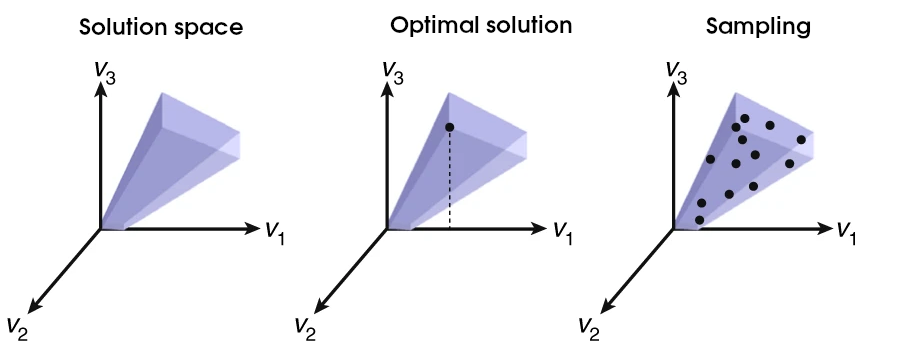
\includegraphics[width=.9\textwidth]{figures/solution_spaces_transparent.png}
         \caption[Flux sampling compared to FBA]{A visual comparison of the insight FBA ("Optimal solution") and flux sampling ("Sampling") return}
         \label{fig:spaces}
      \end{figure}


      Flux sampling has been proved rather valuable for a great range of applications;
      from design experiments and studying enzymopathies~\citep{price2004uniform}
      to the study of metabolism under changing environmental conditions~\citep{herrmann2019flux}
      and the discovery of strain-dependent differences 
      that affect the aroma production in wine yeasts~\citep{scott2021metabolic}. 
      
      Implementations of Markov Chain Monte Carlo algorithms such as 
      Hit-and-Run (HR)~\citep{smith84},  
      the Artificial Centering Hit-and-Run
      (ACHR)~\citep{kaufman1998direction} 
      and Coordinate Hit-and-Run with Rounding
      (CHRR)~\citep{Haraldsdottir17}
      have been adopted and used to a great extent. 
      Similarly to FBA, flux sampling algorithms, e.g. CHRR, have been integrated in \texttt{cobra}~\citep{heirendt2019creation},
      the most widely used 
      software package for metabolic network analysis.
      % Further introductory concepts of MCMC are available at Appendix~\ref{subsec:mcmc_intro}

      On top of that, over the last few years, flux sampling has been 
      used in computational approaches for inferring microbial interactions 
      The Computation Of Microbial Ecosystems in Time and Space (COMETS) project and software~\citep{dukovski2021metabolic}
      first focused on the interactions between a single species and its environment. 
      Nowdays, metabolic modeling moves to the community level. 
      Approaches such as the one of \citeauthor{diener2020micom} in their \texttt{MICOM}
      software~\citep{diener2020micom}, set a new era for the study of microbial ecology. 
      
      
      However, flux sampling is rather challenging from the computational point of view. 
      The "dimensionality curse" is not a problem to a small GEM such as those of single bacterial taxa.
      However, to more complex species and especially in the case of community modeling 
      the dimesion of the derived polytope can be notably high. 
      Moreover, polytopes derived from metabolic networks are usually rather skinny,
      partially due to the great range the various flux values may get, 
      making mixing hard and 
      adding extra complexity~\citep{Haraldsdottir17,schellenberger2009use}. 


      
% SECTION 7 - first draft ready
\section{Aims and objectives}

   The key role of bioinformatics on microbial ecology studies
   was described in the previous chapters and especially 
   when it come to HTS - oriented challenges. 
   The potentials of addressing a subset of these challenges was also 
   described. 
   As HTS technologies become better and better 
   (lower cost, higher accuracy)
   and HTS data become more and more available, 
   efforts to overcome these issues 
   are undoubtedly of great importance. 


   The aim of this PhD was double:
   \begin{enumerate}
      \item to enhance the analysis of microbiome data 
            by building algorithms and software 
            that address limitations and on-going computational challenges
      \item to exploit state-of-the-art methods to identify taxa and functions  
            that play a key part in microbial community assemblages in hypersaline sediments.
   \end{enumerate}
   All parts of this work are purely computational. 
   Both samples and their corresponding sequencing data used in Chapter~\ref{cha:swamp} have been collected 
   and produced by 
   \href{https://scholar.google.com/citations?user=3zs1rNkAAAAJ&hl=en&oi=sra}{Dr. Christina Pavloudi} \footnote{
      \href{https://scholar.google.com/citations?user=3zs1rNkAAAAJ&hl=en&oi=sra}{
         https://scholar.google.com/citations?user=3zs1rNkAAAAJ\&hl=en\&oi=sra
      }
   }. 

   In \textbf{Chapter~\ref{cha:2}}, challenges derived from the analysis of HTS amplicon data are examined.
   A bioinformatics pipeline, called \texttt{PEMA}, for the analysis of several marker genes was developed, combinining several new technologies that allow large scale analysis of hundreds of samples. 
   In addition, a software tool called \texttt{darn}, was built to investigate the unassigned sequences in amplicon data of the COI marker gene. 

   In \textbf{Chapter~\ref{cha:prego}}, data integration, data mining and text-mining methods were exploited to build a knowledge-base, called \texttt{prego}, including millions of associations between:
   \begin{enumerate}
      \item microbial taxa and the environments they have been found in 
      \item microbial taxa and biological processes they occur
      \item environmental types and the biological processes that take place there
   \end{enumerate}

   In \textbf{Chapter~\ref{chap:dingo}}, the challenges of flux sampling in metabolic models of high dimensions was presented along with a Multiphase Monte Carlo Sampling (MMCS) algorithm we developed. 

   In \textbf{Chapter~\ref{cha:swamp}}, sediment samples from a hypersaline swamp in Tristomo, Karpathos Greece were analysed using both amplicon and shotgun metagenomics. 
   The taxonomic and the functional profiles of the microbial communities present there were investigated. 
   Key metabolic processes for ensuring life at such an extreme environment were identified.
   Microbial interactions of the assemblages retrieved were also studied by exploiting 
   data integration and reverse ecology approaches.  

   In \textbf{Chapter~\ref{cha:hpc}}, the history of the IMBBC-HCMR HPC facility was presented indicating the vast needs of computing resources in modern analyses in general and in microbial studies more specifically. 

   Finally, in \textbf{Chapter~\ref{cha:conclusion}}, general discussion and conclusions that have derived from this research were presented. 





% -------------------------
%    NOTES
% -------------------------
% 
%    biotic interactions                  --> cross-feeding of byproduscts, competition for nutrients 
%    confounder (or 'confounding factor') --> something, other than the thing being studied, that could be causing the results seen in a study. 
%                                             confounders have the potential to change the results of research because they can influence the outcomes
%                                             that the researchers are measuring.
%                                             EXAMPLE: we found that people eating red meat have higher possibility for heart issues; but we have to 
%                                                      check whether everyone in the study who ate a lot of red meat may also have smoked cigarettes
%                                                      regularly or been overweight. 
%    circumvented                         --> shortchut, find a way around (an obstacle).
%    stratify                             --> stromatopoio // 
%    stringent                            --> austiros, strict
%    a habitat filtering model supposes that
% habitats with differing environmental
% features support non-overlapping sets of taxa

% The who : microbial diversity
% Only text 

\chapter{Microbial diversity: \textit{who}}
\label{cha:2}

This chapter will be about finding the taxa present in an environment sample. 

First we will discuss a few things about the biodiversity assessment methods in general in terms of a short introduction. 

\section{Metabarcoding..}
Then we will describe PEMA


\begin{figure}{}
   \caption{workflow from publication}
\end{figure}




\section{.. has caveats}
And here we will talk about DARN


\begin{figure}{}
   \centering
   \caption{COI - reference phylogenetic tree}
\end{figure}


\section{What about metagenomics?}


   \subsection{Afoulo-iky}

   \subsection{EOSC Life project}
   And at this point we ll mention our work and 
   findings (if any) in the framework of the EOSC Life project.






%%% Local Variables: 
%%% mode: latex
%%% TeX-master: "thesis"
%%% End: 

% The what and where: ecosystem functioning
% --------------------------------------------------
% 
% This chapter is for PREGO
% 
% --------------------------------------------------


\chapter{Software development to build a knowledge-base at the systems biology level}
\label{cha:prego}



% SECTION 3
\section{PREGO: a literature- and data-mining resource to associate microorganisms, biological processes, and environment types}

Publication relative to this chapter: under submission
\subsection{Introduction}

\subsection{Methods \& Implementation}

\begin{figure}[!htbp]
   \centering
   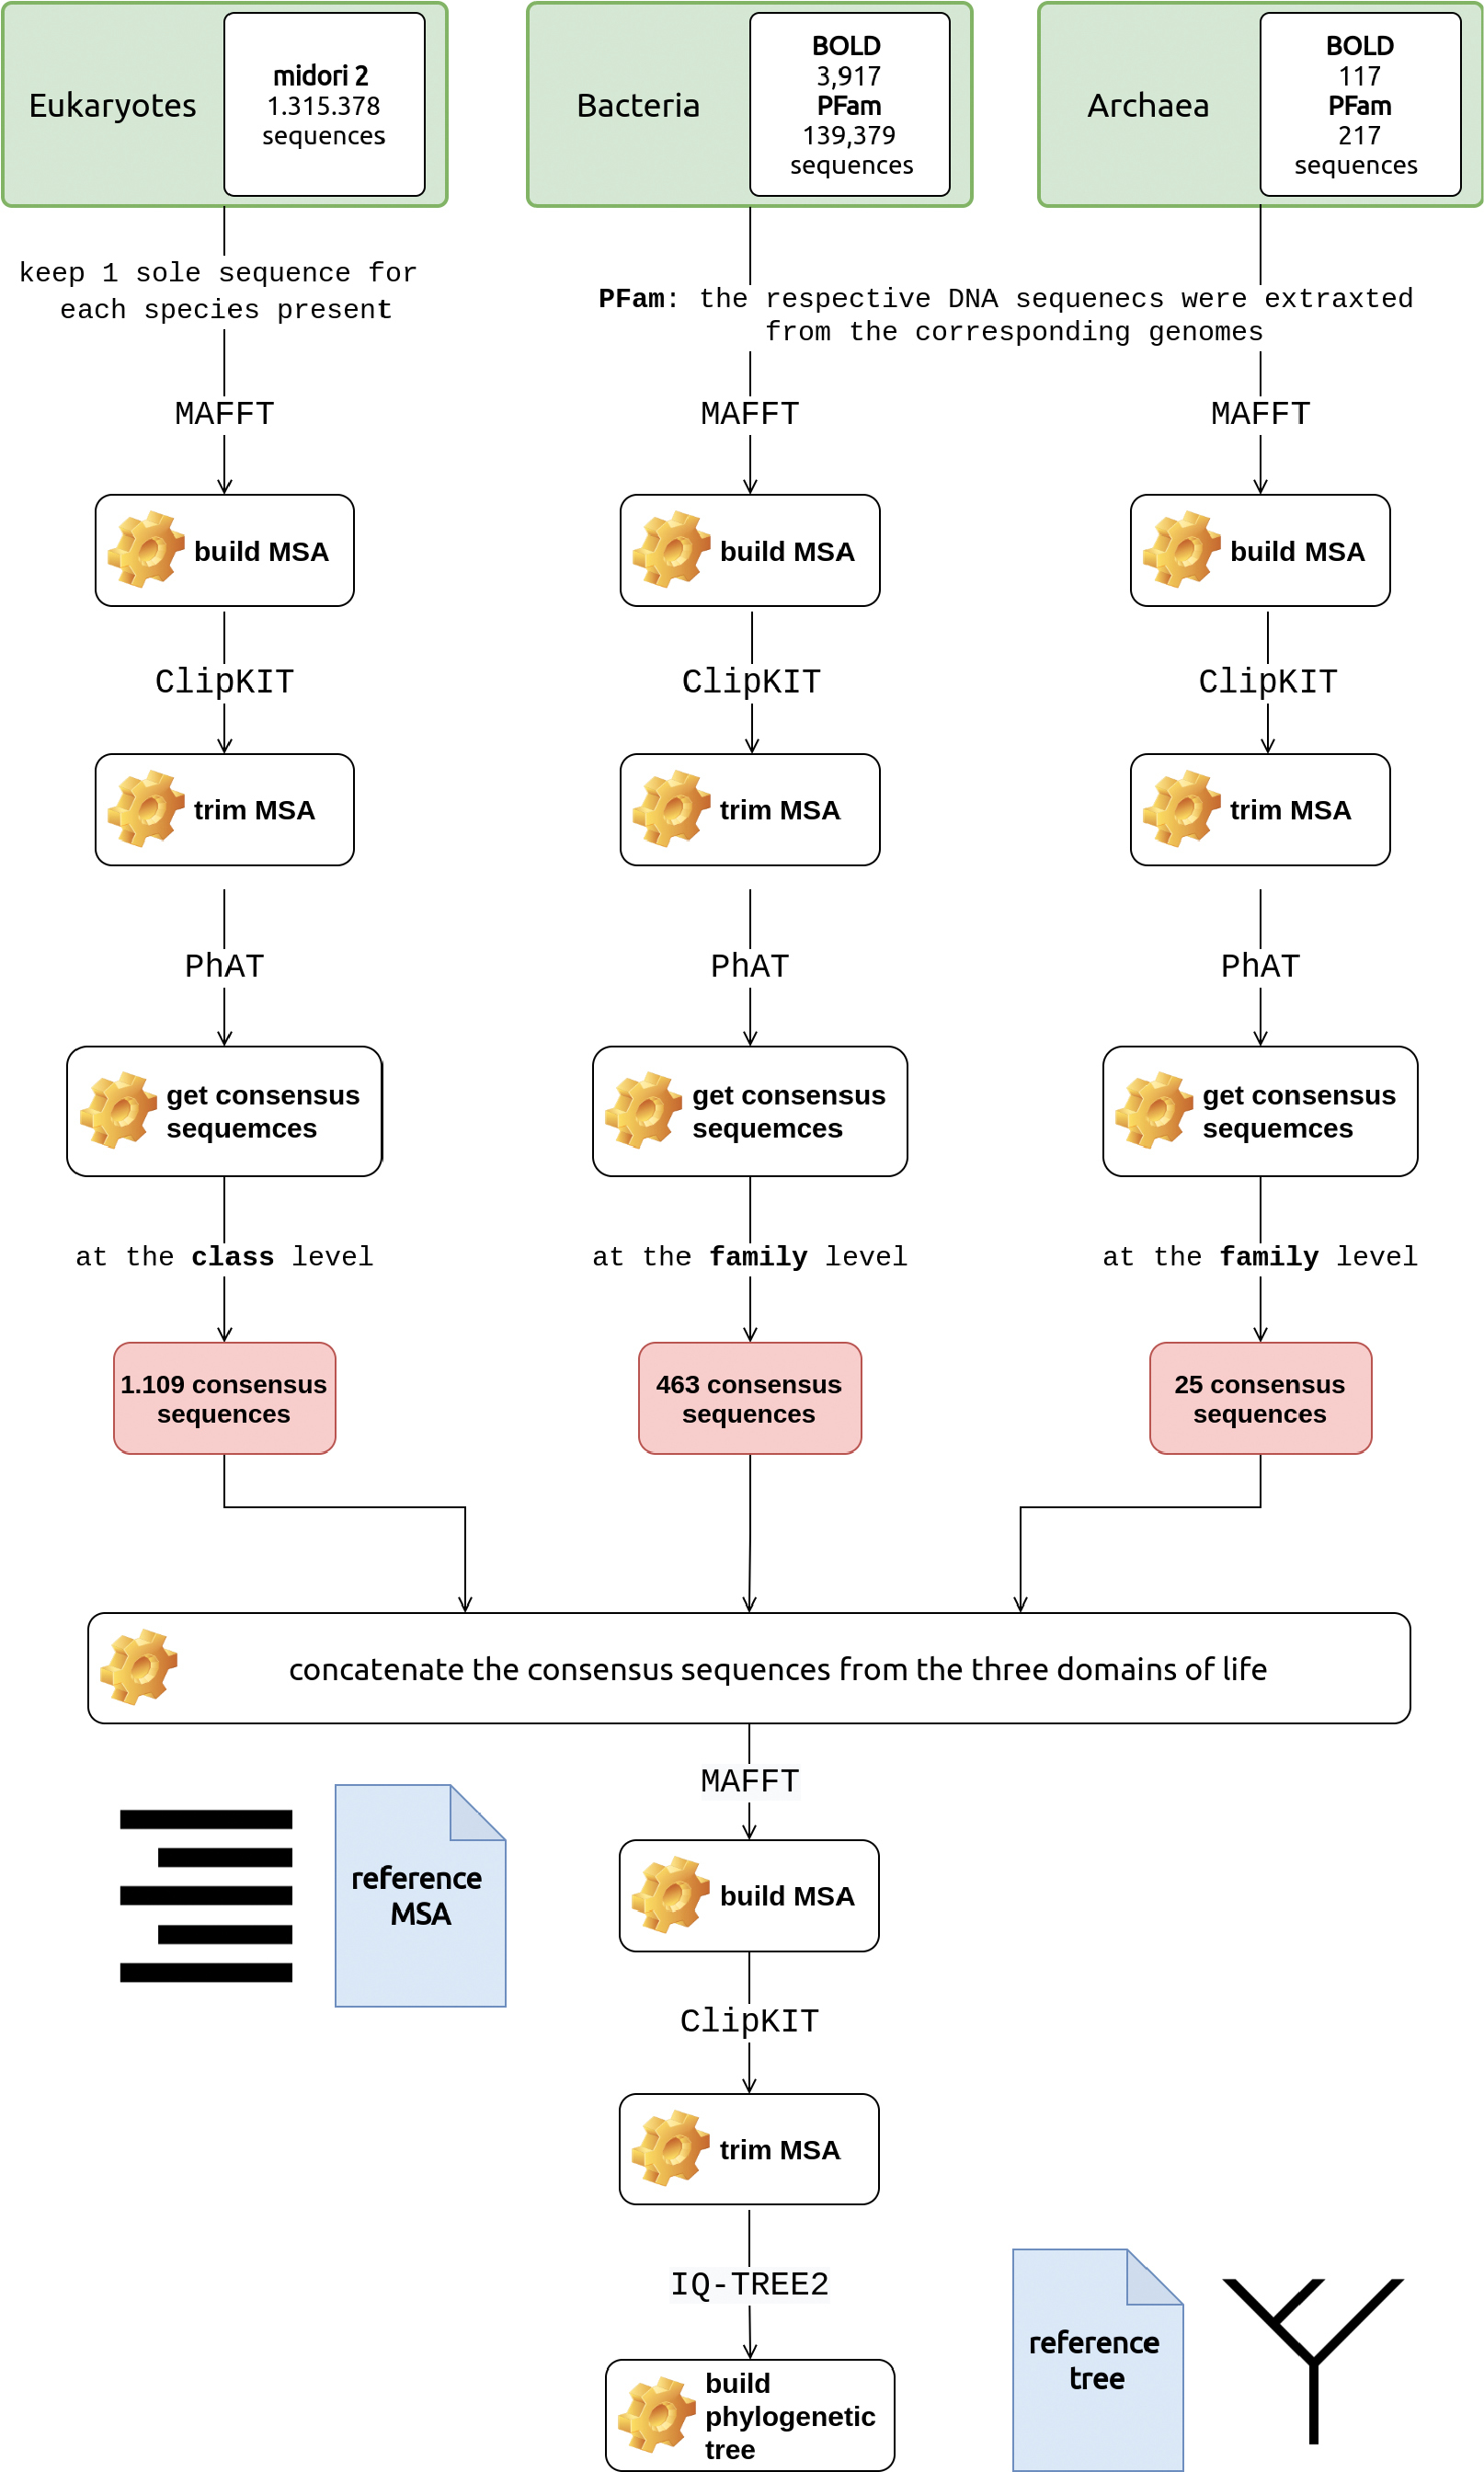
\includegraphics[width=0.75\columnwidth]{figures/darn_methodology.jpg}
   \caption{DARN methodology: figure in the publication}
\end{figure}



\begin{figure}[!htbp]
   \centering
   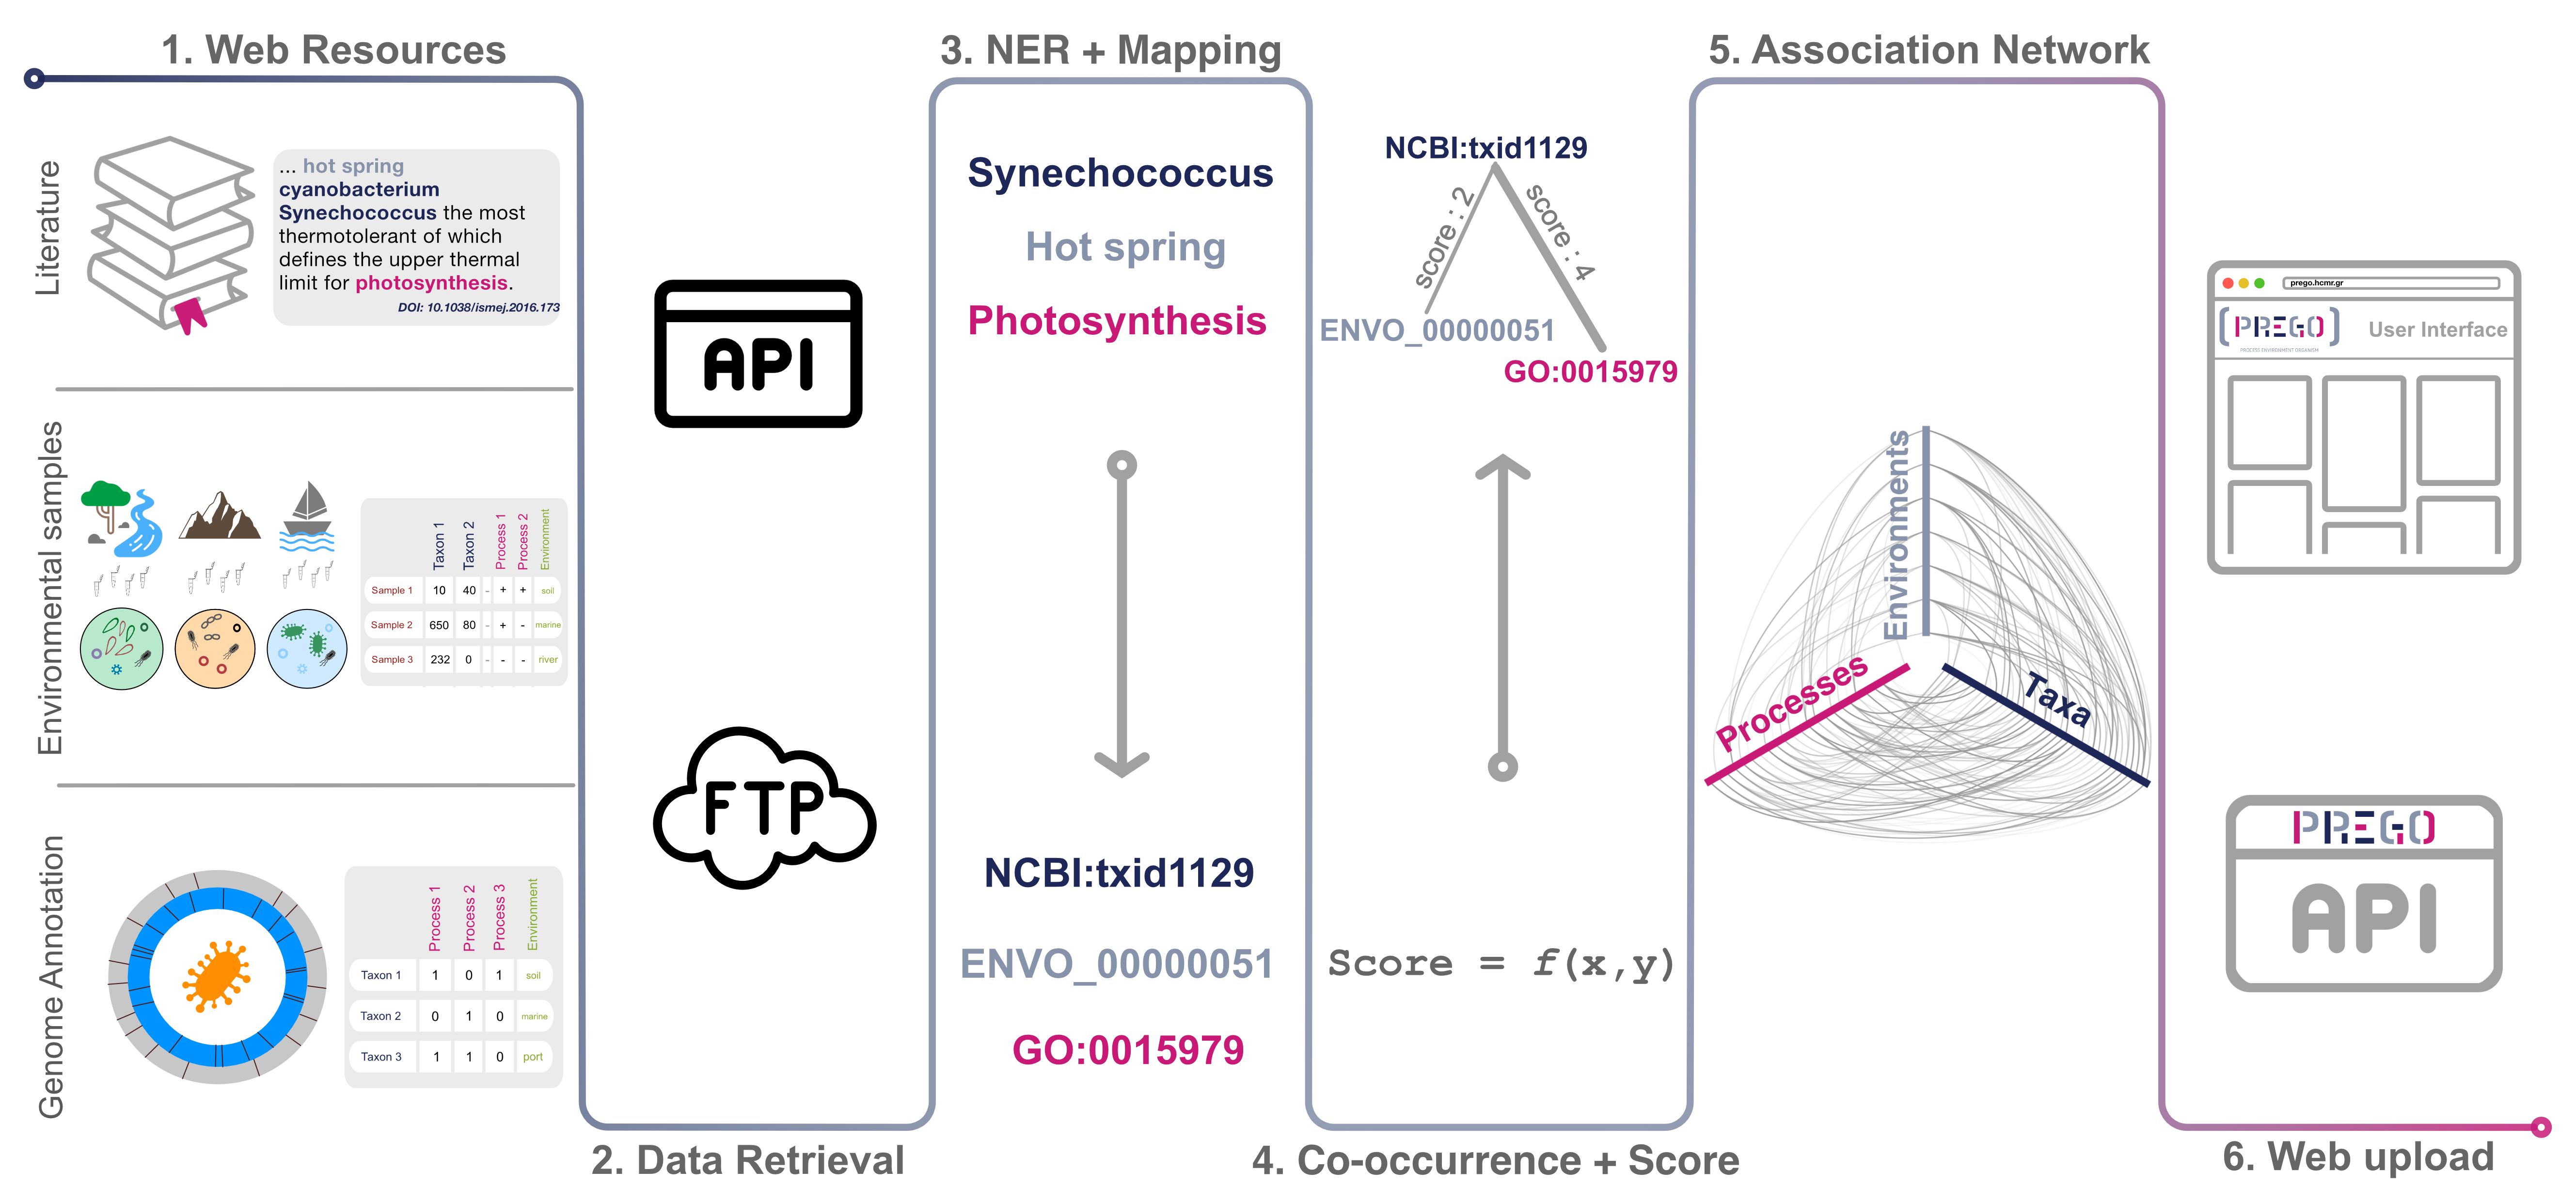
\includegraphics[width=0.98\columnwidth]{figures/prego_analysis_horizontal.png}
   \caption{PREGO methodology: figure in the publication under submission}
\end{figure}

\subsection{Results \& Validation}

\subsection{Discussion}



% The why: microbial interactions
% --------------------------------------------------
% 
% This chapter is for dingo
% 
% --------------------------------------------------

\chapter{Software development to establish metabolic flux sampling 
         approaches at the community level}
\label{cha:dingo}

% ADD AN INTRO FOR THE SECTION

\section{Genome-scale metabolic model analysis}

The relationship between genotype and phenotype is fundamental to biology.
Many levels of control are introduced when moving from one to the other. 
Systems biology aims at deciphering "the strategy" both at the cell and at higher levels of organization, in case of multicell species, that enables organisms to produce orderly adaptive behavior in the face of widely varying genetic and environmental conditions (\cite{strohman2002maneuvering}); the term "strategy" is used as per \cite{polanyi1968life}.
Systems biology approaches aim at interpreting how a system's properties emerge; from the cell to the community level.


\section{A New MCMC Algorithm for Sampling the Flux Space of Metabolic Networks}


\cite{chalki2021SoCG}

% \section{The flux sampling approach}

From \citet{price2004genome} :
"Pairwise correlation coefficients can be calculated
between all reaction fluxes based on uniform random
sampling. Perfectly correlated reactions (R2 = 1) operate
as functional modules within a biochemical network,
whereas uncorrelated reactions (R2 ~0) operate independently of each other. The degree of independence
between reactions is an important consideration when
choosing a set of fluxes to measure that will best determine the operating state of a biochemical network"


Write something from \citeauthor{polanyi1968life}

% \section{The `dingo` Python library}


our approach 

\begin{figure}
   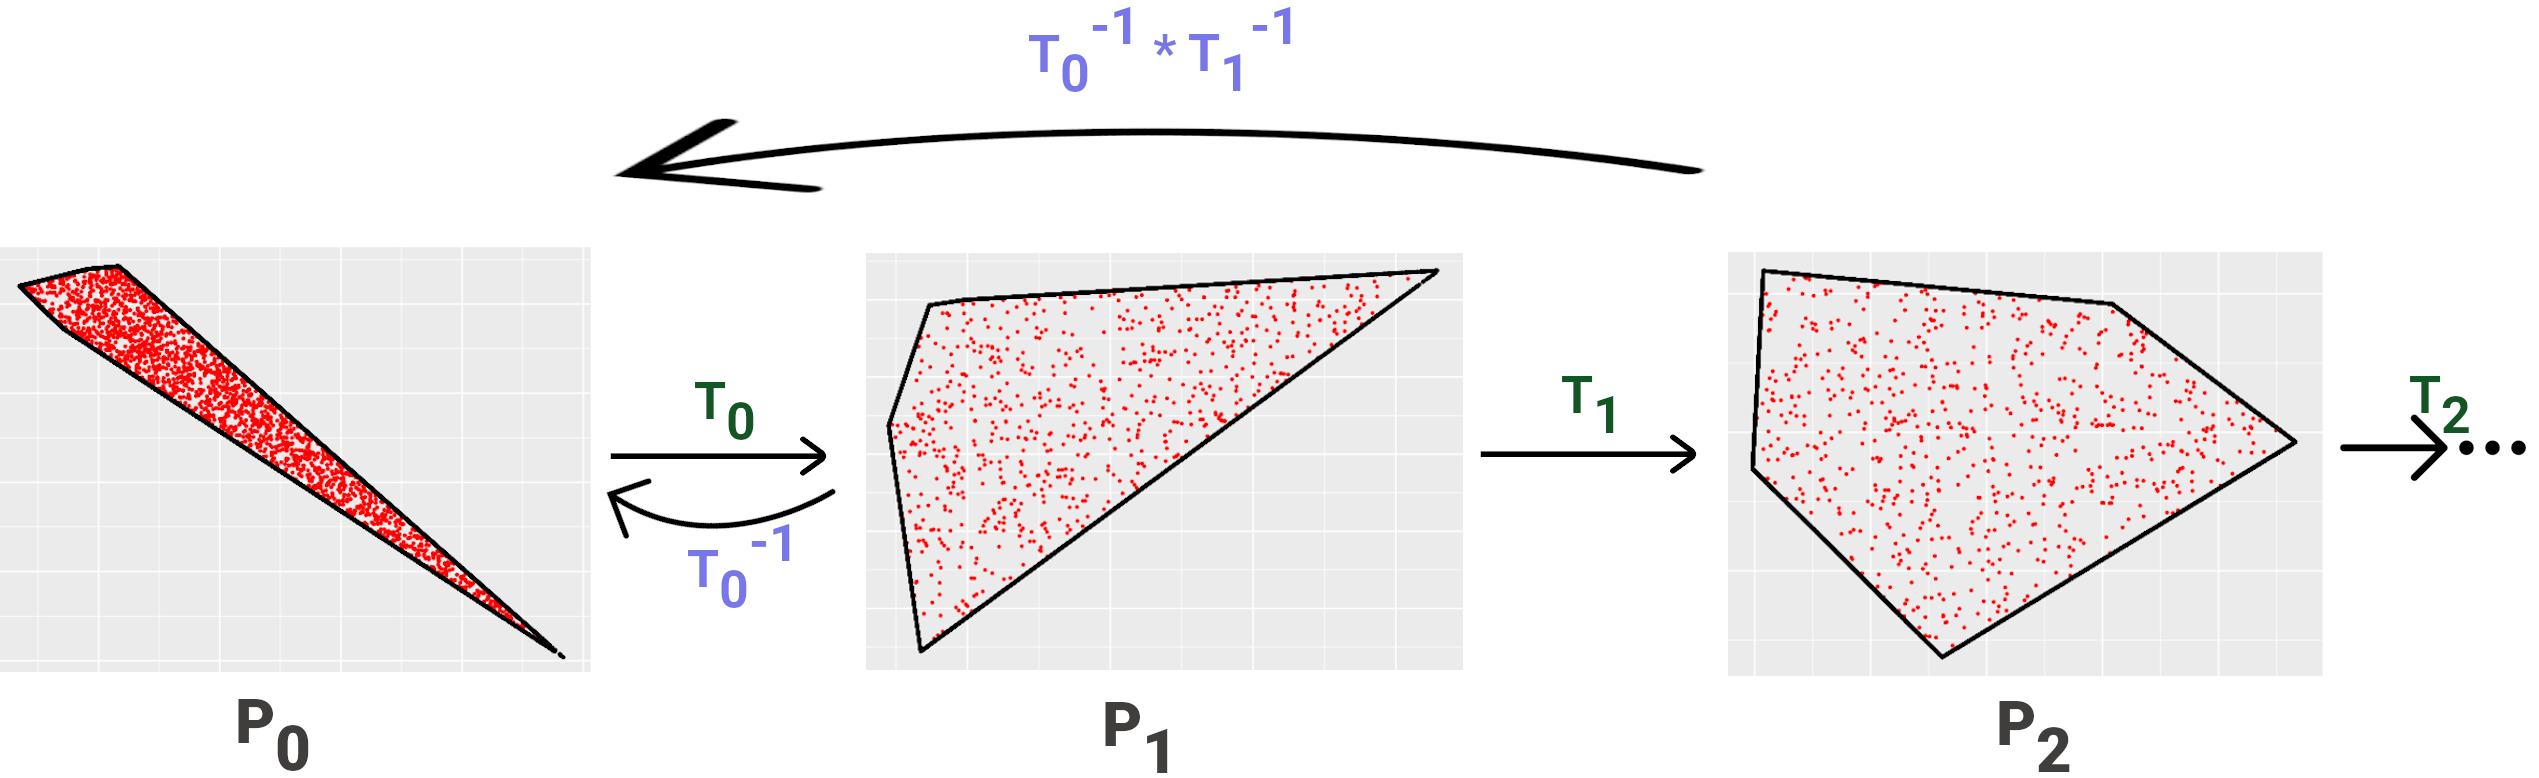
\includegraphics[width=1.0\columnwidth]{figures/sampling_extra_phase_croped.png}
   \caption{Our MMCS algorithm and its first phases}
   \label{fig:mmcs}
\end{figure}


% SECTION 3
\section{Flux sampling at the community level}



%%% Local Variables: 
%%% mode: latex
%%% TeX-master: "thesis"
%%% End: 

% Karpathos case
% --------------------------------------------------
% 
% This chapter is for Tristomo
% 
% --------------------------------------------------

\chapter{
    Studying the microbiome as a whole: the way forward
}
\label{cha:swamp}

Publication relative to this chapter: ongoing work, to be submitted before phd defense, probably not accepted by then though.


% AFOULOPAPER
\section{
   Microbial interactions inference in communities of a hypersaline swamp elucidate mechanisms governing taxonomic \& functional profiles
}

% AFOULOPAPER INTRODUCTION
\subsection{Introduction}



% AFOULOPAPER CONTRIBUTION
\subsection{Contribution}


% AFOULOPAPER METHODS
\subsection{Methods}


   \texttt{darn} and \texttt{PEMA} will be used at this point, among other software 

   \texttt{PREGO} and \texttt{dingo} will be used to this end 



% AFOULOPAPER RESULTS
\subsection{Results}



% AFOULOPAPER DISCUSSION
\subsection{Discussion}







%%% Local Variables: 
%%% mode: latex
%%% TeX-master: "thesis"
%%% End: 

% Computing in bio-research
\chapter{Not the sky, but the computing resources is now the limit}
\label{cha:5}


\section{HPC solutions}

HPC paper


\section{Infrustuctures could be of use}

white paper of Elixir microbiome community 


% Finally... 
\chapter{Conclusion}
\label{cha:conclusion}
The final chapter contains the overall conclusion. It also contains
suggestions for future work and industrial applications.

\lipsum[1-7]

%%% Local Variables: 
%%% mode: latex
%%% TeX-master: "thesis"
%%% End: 


% If there are attachments
\appendixpage*          % indien gewenst
\appendix
% \chapter{PREGO}

\section{Mappings}
\label{app:A}


PREGO produces entity identifiers either by Named Entity Recognition (NER) with the EXTRACT tagger or by mapping retrieved identifiers to the selected ones. 
PREGO adopted NCBI taxonomy identifiers for taxa, Environmental Ontology for environments and Gene Ontology as a structure knowledge scheme for Processes (GObp) and Molecular Functions (GOmfs). 
The latter was for reasons that are two-fold, first Gene Ontology has a Creative Commons Attribution 4.0 License and second there are many resources that have mapped their identifiers to Gene Ontology.
MG-RAST metagenomes and JGI/IMG isolates annotations come with KEGG orthology (KO) terms; 
Struo-oriented genome annotations, on the other hand, have Uniprot50 ids. 
The mapping from KO to GOmf and Uniprot50 to GOmf is implemented via UniProtKB mapping files of their FTP server (see \texttt{idmapping.dat} and \texttt{idmapping\_selected.tab} files). 
By using the 3-column mapping file, the initial annotations were mapped to GOmf. As a complement, a list of metabolism-oriented KEGG ORTHOLOGY (KO) terms has been built (see \textit{prego\_mappings} in the Availability of Supporting Source Codes section).
Finally, as STRUO annotations refer to GTDB genomes, \href{http://ftp.tue.mpg.de/ebio/projects/struo/GTDB_release89/metadata/}{publicly available mappings} (accessed on 24 December 2021) were used to link the genomes used with their corresponding NCBI Taxonomy entries.



\section{Daemons}
\label{app:B}

An important component PREGO approach (Figure A1) is the regular updates which keep PREGO in line with the literature and microbiology data advances. 
The updates are implemented with custom scripts called daemons that are executed regularly spanning from once a month up to six-month cycles. 
This variation occurs because of the API requirements of each web resource as well as the computational intensity of the association extraction from the retrieved data.

\begin{figure}[ht]
   \centering
   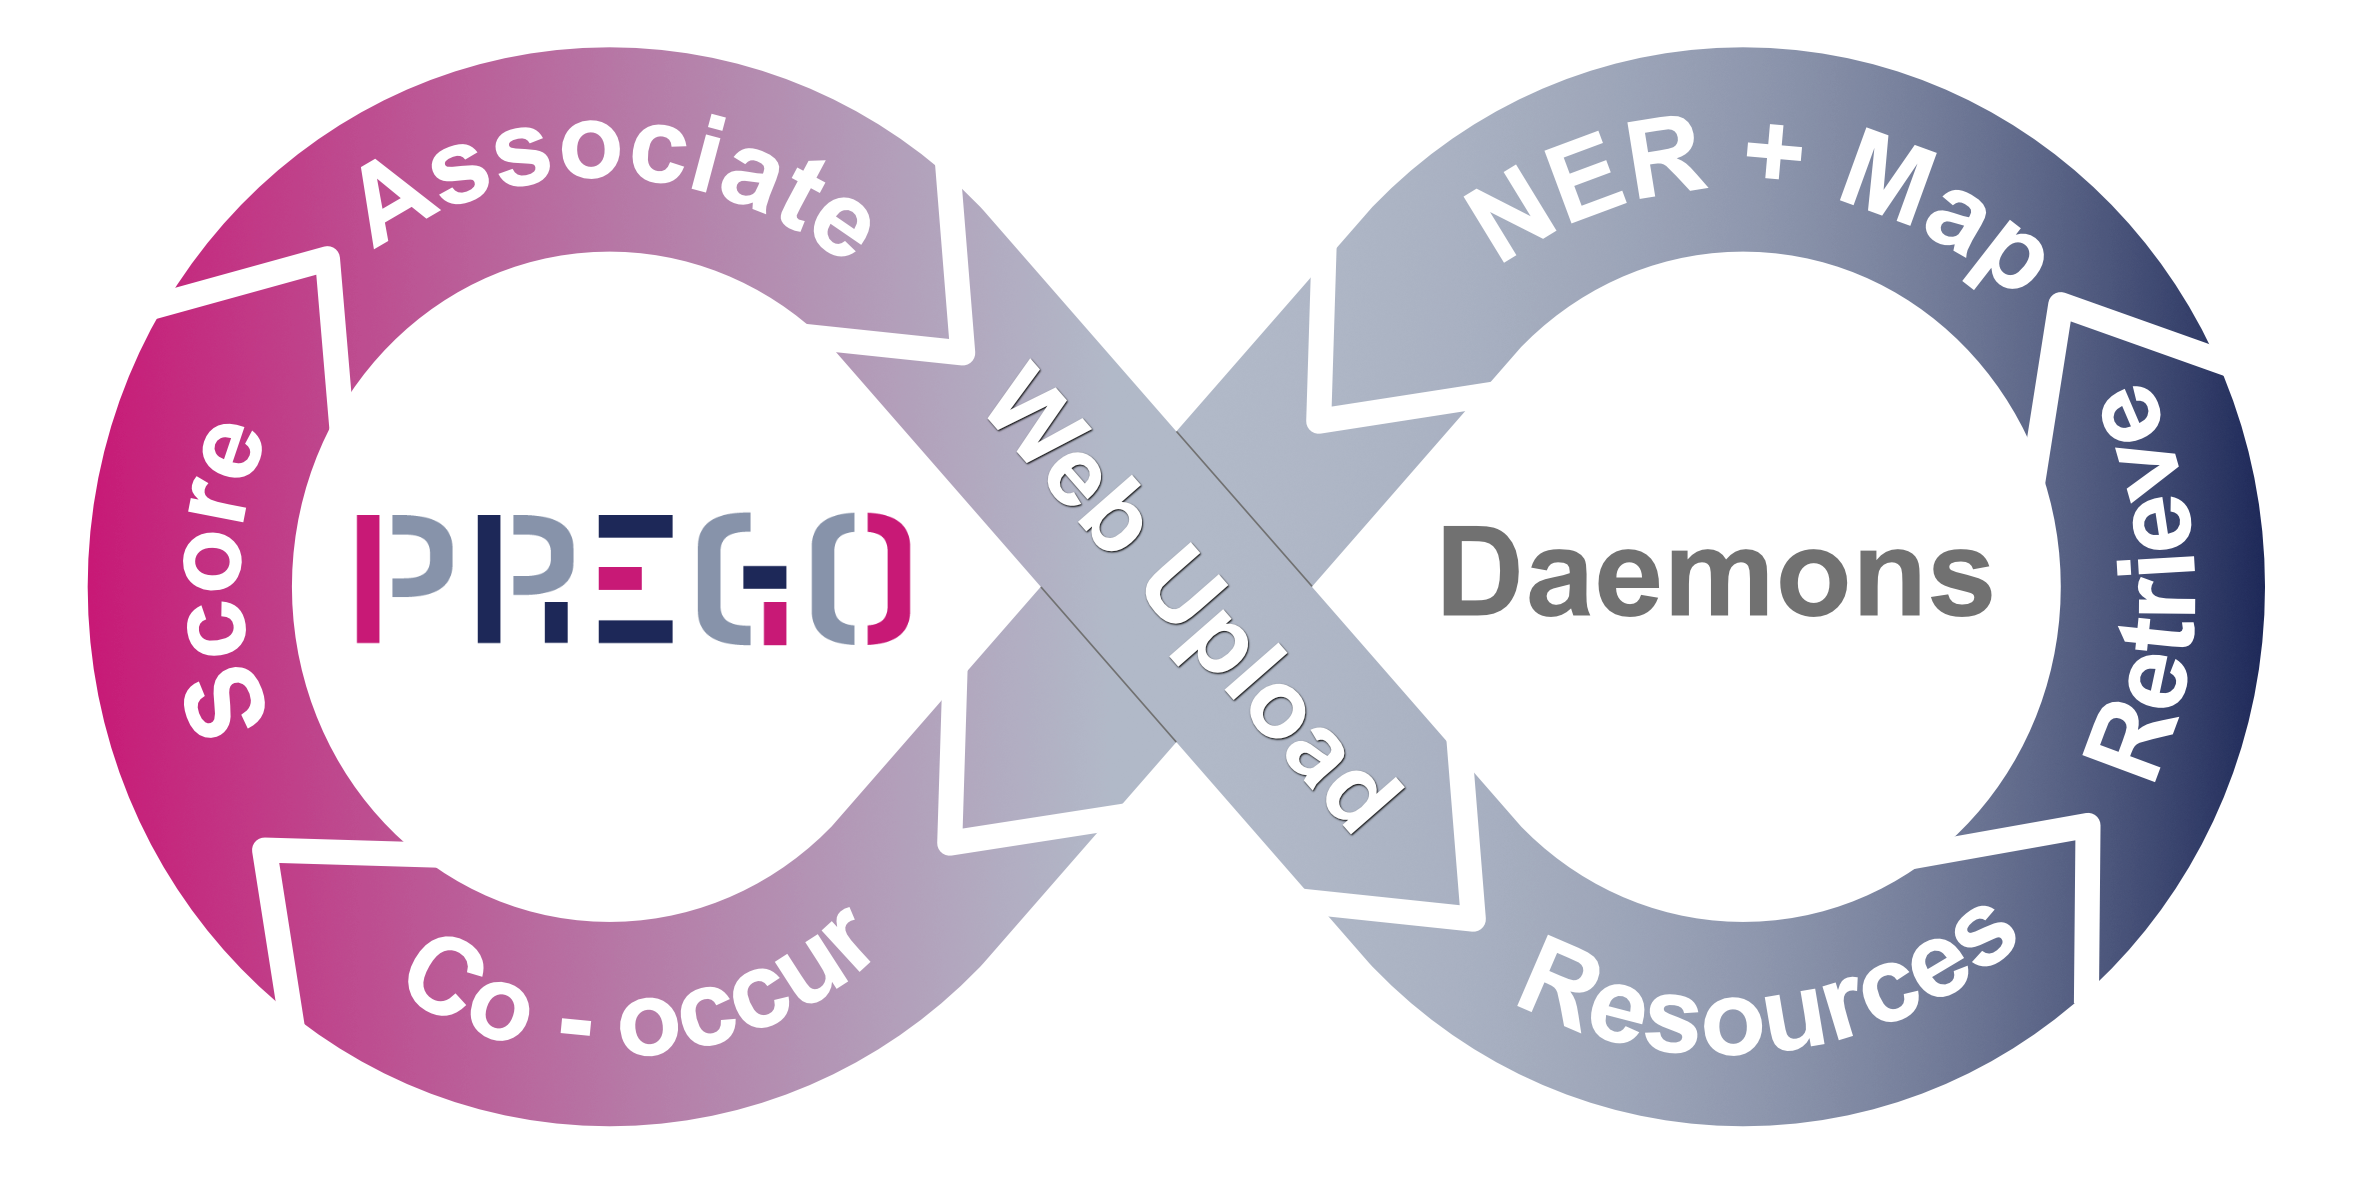
\includegraphics[width=95mm]{figures/figure_A1_PREGO_daemons.png}
   \caption[PREGO DevOps]{Software daemons perform all steps of the PREGO methodology in a continuous manner similar to the Continuous Development and Continuous Integration method.}
   \label{fig:devops}
\end{figure}


Each Daemon is attached to a resource because its data retrieval methods (API, FTP) and following steps, shown in Figure A1, require special handling and multiple scripts (see \textit{prego\_daemons} in the Availability of Supporting Source Codes section).

\section{Scoring}
\label{app:C}


Scoring in PREGO is used to answer the questions:
\begin{itemize}
   \item Which associations are more thrustworthy?
   \item Which associations are more relevant to the user's query?
\end{itemize}

Relevant, informative, and probable associations are presented to the user through the three channels that were discussed previously. 
Each channel has its own scoring scheme for the associations it contains and all of them are fit in the interval $(0,5]$ to maintain consistency. 
The values of the score are visually shown as stars. 
The Genome Annotation and Isolates channel has fixed values of scores depending on the resource because Genome Annotation is straightforward, and the microbe id is known a priori. 
On the other hand, Environmental Samples channel data are based on samples, which contain metagenomes and OTU tables. 
Thus, it has two levels of organization, microbes with metadata, and sample identifiers. Each association of two entities is scored based on the number of samples they co-occur. 
A Literature channel scoring scheme is based on the co-mention of a pair of entities in each document, paragraph, and sentence. The differences in the nature of data require different scoring schemes in these channels.
The contingency table (Table~\ref{table:pregoA1}) of two random variables, $X$ and $Y$ are the starting point for the calculation of scores. The term $X = 1$ might be a specific NCBI id and $Y = 1$ a ENVO term. 
The $c_{1,1}$ is the number of instances that two terms of $X = 1$ and $Y = 1$ are co-occurring, i.e., the joint frequency. 
The marginals are the $c_{1,.}$ and $c{.,1}$ for $x$ and $y$, respectively, which are the backgrounds for each entity type. 
Different handling of these frequencies leads to different measures. 
There is not a perfect scoring scheme, just the one that works best on a particular instance. 
Consequently, scoring attributes require testing different measures and their parameters.



\begin{table}[ht]
   \centering
   \begin{tabular}{c|llll}
    & \multicolumn{4}{l}{Y = y} \\ \cline{2-5} 
   \multirow{4}{*}{X = x} &  & Yes & No & Total \\ \cline{3-5} 
    & \multicolumn{1}{l|}{Yes} & $c_{x,y}$ & $c_{x,0}$ & $c_{x,.}$ \\
    & \multicolumn{1}{l|}{No} & $c_{0,y}$ & $c_{0,0}$ & $c_{0,.}$ \\
    & \multicolumn{1}{l|}{Total} & $c_{.,y}$ & $c_{.,0}$ & $c_{.,.}$
   \end{tabular}
   \caption[PREGO contingency table between two terms]{Contingency table of co-occurrences between entities $X = x$ and $Y = y$. 
   This is the basic structure for all scoring schemes. $c_{x,y}$ is the count of the co-occurrence of these entities. $c_{x,.}$ is the count of the $x$ with all the entities of $Y$ type (e.g., Molecular function). Conversely, $c_{.,y}$ is the count of $y$ with all the entities of $X$ type (e.g., taxonomy}
   \label{table:pregoA1}
\end{table}


\section*{Literature Channel}

Scoring in the Literature channel is implemented as in STRING 9.1 \citep{franceschini2012string} and COMPARTMENTS \citep{binder2014compartments}, where the text mining method uses a three-step scoring scheme. 
First, for each co-mention/co-occurrence between entities (e.g., Methanosarcina mazei with Sulfur carrier activity), a weighted count is calculated because of the complexity of the text.  


\begin{equation}
   c_{x,y} = \sum_{k=1}^{n}{w_d \delta_{dk}(x,y) +w_p \delta_{p,k}(x,y) + w_s \delta_{sk}(x,y)}
   \label{eq:prego-score-1}
\end{equation}



Different weights are used for each part of the document ($k$) for which both entities have been co-mentioned, $w_d = 1$ for the weight for the whole document level, $w_p = 2$ for the weight of the paragraph level, and $w_s = 0.2$ for the same sentence weight. 
Additionally, the delta functions are one (Equation~\ref{eq:prego-score-1}) in cases the co-mention exists, zero otherwise. Thus, the weighted count becomes higher as the entities are mentioned in the same paragraph and even higher when in the same sentence.
Subsequently, the co-occurrence score is calculated as follows:

\begin{equation}
   score_{x,y} = c_{x,y}^a (\frac{c_{x,y} c_{.,.}}{c_{x, .}c_{.,y}})^{1-a}
   \label{eq:prego-score-2}
\end{equation}
   


where $a = 0.6$ is a weighting factor, and the $c_{x,.}$, $c_{.,.}$, 
$c_{.,y}$ are the weighted counts as shown in Table~\ref{table:pregoA1} estimated using the same Equation~\ref{eq:prego-score-2}. 
This value of the weighting factor has been chosen because it has been optimized and benchmarked in various applications of text mining [34,70,71]. 
The value of Equation~\ref{eq:prego-score-2} is sensitive to the increasing size of the number of documents (MEDLINE PubMed—PMC OA).
Therefore, to obtain a more robust measure, the value of the score is transformed to $z$-score. 
This transformation is elaborated in detail in the COMPARTMENTS resource \citep{binder2014compartments}. 
Finally, the confidence score is the $z$-score divided by two. Cases in which the scores exceed the (0,4] interval are capped to a maximum of 4 to reflect the uncertainty of the text mining pipeline.

\section*{Environmental Samples Channel}

Data from environmental samples are OTU tables and metagenomes. Thus, for each entity x, the number of samples is calculated as the background and a number of samples of the associated entity (metadata background) c.,y (see Table A1). Each association between entities x, y has a number of samples, cx,y that they co-occur. Note that each resource is independent and the scoring scheme is applied to its entities. This means that the same association can appear in multiple resources with different scores. The score is calculated with the following formula:

\begin{equation}
   score_{x,y} = 2.0*\sqrt{\frac{c_{x,y}}{c_{.,y}}}^{ \:a}
\end{equation}


This score is asymmetric because the denominator is the marginal of the associated entity. 
Thus, the score decreases as the marginal of $y$ is increasing, i.e., the number of samples that $y$ is found. 
On the other hand, it promotes associations in which the number of samples of the association are similar to the marginal of $y$. 
The exponents on the numerator and denominator equal to $0.5$ and 
to $0.1$, respectively, in order to reduce the rapid increase of score.
Lastly, the value of the score is capped in the range $(0,4]$.


\section{Bulk download}
\label{app:D}

Users can also download programmatically all associations per channel through the links that are shown in Table~\ref{table:prego-appD-1}. 
The data are compressed to reduce the download size and md5sum files are provided as well for a sanity check of each download.

% PREGO BULK DOWNLOAD TABLE 
\begin{table}[ht]
   
   \begin{adjustwidth}{-2cm}{}

   \begin{tabular}{llll}
   \toprule
   Channel & Link & md5sum & Size (in GB) \\ \midrule

   Literature & \href{https://prego.hcmr.gr/download/literature.tar.gz}{literature.tar.gz} & \href{https://prego.hcmr.gr/download/literature.tar.gz.md5}{literature.tar.gz.md5} & 5.4 \\

   \begin{tabular}[c]{@{}l@{}}Environmental \\ Samples\end{tabular} &
   \href{https://prego.hcmr.gr/download/environmental\_samples.tar.gz}{environmental\_samples.tar.gz} & 
   \href{https://prego.hcmr.gr/download/environmental\_samples.tar.gz.md5}{environmental\_samples.tar.gz.md5}
   & 0.69 \\

   \begin{tabular}[c]{@{}l@{}}Annotated \\ genomes and \\ isolates\end{tabular} & 
   \href{https://prego.hcmr.gr/download/annotated\_genomes\_isolates.tar.gz}{annotated\_genomes\_isolates.tar.gz} &
   \href{https://prego.hcmr.gr/download/annotated\_genomes\_isolates.tar.gz.md5}{annotated\_genomes\_isolates.tar.gz.md5} & 0.26 \\ \bottomrule
   \end{tabular}
   \end{adjustwidth}
   \caption[PREGO Bulk download links and md5sum files.]{Bulk download links and md5sum files.}
   \label{table:prego-appD-1}
\end{table}
% \chapter{The Last Appendix}
\label{app:n}
Appendices are numbered with letters, but the sections and subsections use
arabic numerals, as can be seen below.

\section{Lorem 20-24}
\lipsum[20-24]

\section{Lorem 25-27}
\lipsum[25-27]

%%% Local Variables: 
%%% mode: latex
%%% TeX-master: "thesis"
%%% End: 


\backmatter 

% The bibliography is placed after the appendices.
% You can replace the default "abbrv" bibliography style with another.
% \bibliographystyle{alpha}
\bibliographystyle{ieeetr.bst}
\bibliography{references}

\end{document}

%%% Local Variables: 
%%% mode: latex
%%% TeX-master: t
%%% End: 
